% Chapter Template

\chapter{Convolutional Neural Networks} % Main chapter title
\label{ChapterCNN}

\epigraph{\textit{Aiutiamoli a fare da soli!}\newline
\footnotesize{\textit{Let's help them to do themselves!}}}{--- \textup{Maria Montessori}}

% TODO: manca universal approximation theorem (da pagg 194 e seguenti del deeplearningbook)

In this chapter we explore a new strategy to perform profiling SCAs, addressing the misalignment issue and endorsing the Deep Learning (DL) paradigm. To this aim we present results published in \cite{DBLP:conf/ches/CagliDP17}, where Convolutional Neural Networks are proposed to help against misalignment-oriented countermeasures. Actually, the term Time-Delay Neural Network (TDNN) would be more appropriated than Convolutional Neural Network. Indeed the TDNNs  \cite{lang1990time} consist in the Convolutional Neural Networks applied to one-dimensional data, as side-channel traces are. Nevertheless, the fame that CNNs reached in last years, and especially since 2012, where a CNN architecture (the \textquotedbl AlexNet\textquotedbl) \cite{KSH12}  won the \emph{ImageNet Large Scale Visual Recognition Challenge}, a large-impact image recognition contest, leads to the disappearing of term TDNN from DL literature. Today, to specify the architecture of a TDNN in the most common DL libraries, one needs to exploit functionalities related to the CNNs' architecture, specifying \eg that one of the input dimensions equals 1. For these reasons we kept the term CNN for our discussion. 

\section{Motivation}
The context we choose to study DL techniques, and CNNs in particular, is the one of cryptographic implementations protected by countermeasures aiming at enhancing misalignment or desynchronisation in side-channel acquisitions. The latter countermeasures are either implemented in hardware (random hardware interruption or non deterministic processors \cite{irwin2002instruction,may2001non}, unstable clock \cite{moore2002improving,moore2003balanced}) or in software (insertion of random delays through dummy operations \cite{coron2009efficient,coron2010analysis}, shuffling \cite{veyrat2012shuffling}). Techniques analysed in previous chapters were applied in contexts where acquisitions were perfectly synchronous, and are not able to well extend to desynchronised context, as briefly observed in Secs.~\ref{sec:misalignment} and \ref{sec:KDAdrawbacks}.\\

Desynchronisation might be seen as a noise component of the acquisitions, as done in the leakage model proposed in \cite{chari1999towards}. Anyway, it raises the noise that hides sensitive information in the traces. From a statistical point of view, a theoretically satisfying answer to such a noise raise is the solely augmentation of the number of acquisitions: if the attack strategy, in terms of exploited statistical tools, keeps unchanged, increasing the acquisitions by a factor which is somehow linear in the misalignment effect, as discussed in \cite{mangard2004hardware}, might suffice to let the attack be as effective as in the synchronous case. In practice, such an augmentation might be unacceptable for many reasons. First, an attacker or evaluator might have a time or memory bound for the acquisition campaign. Second, the attacked device might implement a security defence denying an unlimited number of executions. Third, attack routines might suffer, in terms of complexity, more than linearly from a raising of the number of  data to be treated, \eg the KDA search for a non-linear feature extraction has a complexity that grows in a cubic way with the number of traces.  \\

The second approach proposed in the SCA literature to deal with misaligned trace sets consists in applying a realignment preprocessing before the attack. Two realignment techniques families might be distinguished: a signal-processing oriented one (\eg \cite{nagashima2007dpa,van2011improving}), more adapted to hardware countermeasures, and a probabilistic-oriented one (\emph{e.g.} \cite{durvaux2012efficient}), conceived for the detection of dummy operations, \emph{i.e.} software countermeasures. \\

We found in Convolutional Neural Networks the possibility of performing a profiling attack in an end-to-end form, directly extracting sensitive information from rough data, without applying any realignment preprocessing. We believe that realignments, a well as dimensionality reduction techniques, as discussed in Sec.~\ref{sec:KDAdrawbacks}, bring with them the risk of corrupting useful information in data. Indeed a realignment process acts modifying signals with the goal of obtaining some well-synchronised dataset, making traces be somehow similar to each other. On one hand it is not trivial to evaluate the accuracy of a realignment, thus to establish if a performed preprocessing is satisfying. On the other hand, the goal of a realignment is not extracting sensitive and discriminant information from traces. Even if we were able to affirm that a resynchronisation is somehow  perfect, by means of some special metrics, nothing guaranties that in the attempt of realigning the trace set the useful information is not discarded. Nowadays, CNNs and DL tools in general are standing out, thanks to their good scalability to \textquotedbl big-data\textquotedbl context. One of their strength is that they are easily parallelisable, and can easily exploit computational facilities as GPUs (or the so-called \emph{TPU - Tensor Processing Units} developed by purpose for NNs), allowing computational accelerations. As we have seen in Sec.~\ref{sec:overfitting}, the higher amount of data are available, the higher capacity is admissible for a ML model, without incurring in overfitting, and higher capacity corresponds to the possibility of learning more complex problems. From this point of view, the success of NNs in last years is mainly due to the always increasing amount of available data, and to their scalability. However, even in contexts where a lack of data may occur, \eg side-channel contexts in which the number of acquisitions may be limited, a stratagem exists in ML literature, under the name of Data Augmentation (DA), that may allow high capacity NNs avoid overfitting and perform well. 

\section{Introduction}
Machine Learning approaches often decline in multiple preprocessing phases such as data realignment, feature selections or dimensionality reduction, followed by a final model optimisation. This is the case even for the SCA routines that we considered in previous chapters, or for SCAs that apply realignment preprocessing. Deep Learning is a branch of Machine Learning whose aim is to avoid any preliminary preprocessing step from the model construction work-flow. For example, in Deep Learning the data dimensionality reduction is not necessarily explicitly performed by a distinct learned  function $\extract$. On the contrary, they directly and implicitly extract interesting features, possibly realign data, and estimate the opportune model to solve the task. The model is searched in a family of models that are composed by a cascade of parametrisable layers, which may be optimised in a single global learning process. Such models are called \emph{Artificial Neural Network}, or simply \emph{Neural Networks} (NNs). 

\subsection*{Solution for the KDA Drawbacks}
By construction, NNs are the ML answer to the drawback of work-flows we analysed in previous chapters and discussed as \emph{two-phased approach drawback} in last section of Chapter~\ref{ChapterKernel}. Actually, NNs are answers to other drawbacks pointed out in the same section. \\

In particular NNs are not memory-based. This implies that, after the training phase whose computational complexity is influenced by the size of the training set, they do not need to access the training set any more. By consequence, the obtained model is in general faster in processing new data, than techniques obtained \via kernel machines, for which the training traces themselves are part of the model parameters. This property belongs to the characteristics allowing NNs to be easily scalable to huge training sets.\\

Finally, we pointed out as drawback of techniques analysed in previous chapters their weakness to trace misalignment. Since the CNNs has been developed to treat difficulties as misalignments, scaling, rotations, etc. usually met in image processing,  we claim in this chapter, and verify through various experiments, that such CNNs provide an attack strategy that can keeps effective in presence of misalignment countermeasure. 

\subsection*{Organisation of the Chapter}
In Sections \ref{sec:MLP} and \ref{sec:learningAlgorithm}, notions of DL are introduced. In particular the common classification-oriented \emph{Multi-Layer Perceptron} model is described together with the common practices to train it. The way we exploit NNs to perform SCAs is described in Sec.~\ref{sec:attackNN}, while the performance metrics we will use for experiments are given in Sec.~\ref{sec:performances_NN}. A description of the CNN models is provided in Sec.~\ref{sec:CNN} while the Data Augmentation techniques that we will exploit are introduced in Sec.~\ref{sec:DA}.  Finally, three sections are dedicated to experiments. We tested the same CNN architecture against three different targets: in Sec.~\ref{sec:soft} we test it against a software countermeasure. In Sec.~\ref{sec:hard} it is tested against a simulated hardware countermeasure, and, in Sec.~\ref{sec:AES}, against a real-case cryptographic implementation protected by an enhanced jitter. 


% The answers to the 3 drawbacks of previous chapter (misalignment, memory complexity and actual number of params, two phases approach)
%"In practice, however, it is often worth investing substantial computational resources during the training phase in order to obtain a compact model that is fast at processing new data" (Bishop intro chap 5)

% RICICLATO DALL'EX CAPITOLO 1
%Kernel techniques like the KDA  are as well inherited from Machine Learning domain and consist in strategies that allow to build interesting extensions of many algorithms. One of their characteristics, that turns to be a drawback to apply them in SCA context is that are memory-based: the entire set of profiling traces, \ie those acquired by observing the open samples, has to be stored and accessed in the attack phase. In this sense they are highly memory-consuming, and quite slow to apply: they do not scale well in presence of huge profiling trace sets as those that are often necessary to perform profiling SCAs. In contrast to them, models provided by Neural Networks (NNs) are Machine Learning solutions that are known to be easily scalable to huge datasets and not memory-based. We decided to explore such an approach and pointed out that it not only provided solutions to tackle such a computational performance drawback.


\section{Neural Networks and Multi-Layer Perceptrons}\label{sec:MLP}
In Chapters~\ref{ChapterIntroductionSCA} and \ref{ChapterIntroML} we highlighted a strong analogy between profiling SCAs and classical ML classification task. Thus, we are interested in the NNs' solutions for the classification task. We recall from Chapters~\ref{ChapterIntroML} that for the classification task, the learning algorithm is asked to construct a function $\MLmodel\colon \mathbb{R}^\traceLength \rightarrow \{0,1\}^{\numClasses}$, where elements of $\sensVarSet$, \ie the set of classes, are here expressed \via the \emph{one-hot encoding} (\ref{sec:notations}). The output of such a function is said to be \emph{categorical}, \ie $\sensVarSet$ is a discrete finite set. A variant of the classification task consists in finding a function $\MLmodel\colon \mathbb{R}^\traceLength \rightarrow [0,1]^{\numClasses}$ defining a probability distribution over classes. We will prefer this last formulation. Often for this task, NNs are exploited to create discriminative models, \ie models that directly approximate the latter function $\MLmodel$ which is actually viewed as the posterior conditional probability of a label given the observed trace. This is the use we propose in this chapter, and it is in opposition to the Template Attack we exploited in previous chapters. Indeed, as described in Sec.~\ref{sec:TA}, a TA is based over the construction of generative models, \ie the approximation of the \emph{templates}, which coincide with the conditional probabilities of the traces given a label. \\

Using NNs the function $\MLmodel$ is obtained by combining several simpler functions, called \emph{layers}. An NN has an \emph{input layer} (the identity over the input datum $\vLeakVec$), an output layer (the last function) and all other layers are called \emph{hidden} layers.  The output of $\MLmodel$ is a $\numClasses$-sized vector $\vNNOutput$ of scores for the $\numClasses$ labels. In general, such a vector might or not represent the approximation of a probability distribution. In our case it will. The nature of the NN's  layers, their number and their dimension in particular, is called the \emph{architecture} of the NN. All the parameters that define an architecture, together with some other parameters that govern the training phase, are its \emph{hyper-parameters}. The so-called \emph{neurons}, that give the name to the NNs, are the computational units of the network and essentially process a scalar product between the coordinates of its input and a vector of  \emph{trainable weights} (or simply \emph{weights}) that have to be \emph{trained}. Each layer processes some neurons and the outputs of the neuron evaluations will form new input vectors for the subsequent layer. As we will see, the trainable weights of a NN are in general those defining the linear operations, which are scalar products processed by the neurons. Neurons can be implemented to operate in parallel and are very efficient to be processed and differentiated on GPUs. \\


The {\em Multi-Layer Perceptrons} (MLPs), or \emph{Feed-forward Neural Networks}, are a family of NN's architectures, associated with a function $\MLmodel$  that is composed of multiple linear functions and some non-linear functions, called {\em activations}. The name \emph{feedforward} refers to the fact that the information flows from  the input to the output, through the intermediate computations, without any feedback connection in which outputs of the model are fed back into itself.  This is in opposition to the so-called \emph{Recurrent Neural Network} structures. The CNNs are a generalisation of the MLPs.  \\

We can express a typical classification-oriented MLP by the following form:
\begin{equation}\label{eq:MLP}
\MLmodel(\vLeakVec) = \softmax\circ\lambda_n\circ\sigma_{n-1}\circ\lambda_{n-1}\circ\dots\circ \lambda_1(\vLeakVec)=\yyy \mbox{ ,}
\end{equation}
where:
\begin{itemize}
\item The $\lambda_i$ functions are typically the so-called \emph{Fully-Connected} (FC) layers and are expressible as affine functions: denoting $\vLeakVec\in\mathbb{R}^D$ the input of an FC, its output is given by $\textbf{A}\vLeakVec + \vec{b}$, being $\textbf{A}\in\mathbb{R}^{D\times C}$ a matrix of weights and $\vec{b}\in\mathbb{R}^C$ a vector of biases. These weights and biases are the trainable weights of the FC layer. They are called \emph{Fully-Connected} because each $i$-th input coordinate is \emph{connected} to each $j$-th output via the $\textbf{A}[i,j]$ weight. FC layers can be seen as a special case of the linear layers in general feedforward networks, in which not all the connections are present. The absence of some $(i,j)$-th connections can be formalized as a constraint for the matrix $\textbf{A}$ consisting in forcing to $0$ its $(i,j)$-th coordinates.

\item  The $\sigma_i$ are the so-called \emph{activation functions} (ACT): an activation function is a non-linear real function that is applied independently to each coordinate of its input. In general it does not depend on trainable weights. We denote them by $\sigma$ since in general they are functions similar to the \emph{logistic sigmoid} introduced in \ref{example:LDA}, which is denoted by $\sigma$ as well: indeed historically sigmoidal functions, \ie real-valued, bounded, monotonic, and differentiable functions with a non-negative first derivative, were recommended. Nevertheless, the recommended function in modern neural network literature is the so-called \emph{Rectified Linear Unit} (ReLU), introduced by \cite{nair2010rectified} and defined as $\mathrm{ReLU}(\vLeakVec)[i] = \max(0,\vLeakVec[i])$. Even if this function is not sigmoidal, not being bounded, nor differentiable, the fact of being a non-linear transformation but still piecewise linear, allows to preserve many of the properties that make linear models easy to optimise with gradient-based method.
 

\item $\softmax$ is the \emph{softmax}\footnote{To prevent underflow, the log-softmax is usually preferred if several classification outputs must be combined.} function (SOFT), already introduced in \ref{example:LDA}: $\softmax(\vLeakVec)[i] = \frac{e^{\vLeakVec[i]}}{\sum_{j}e^{\vLeakVec[j]}}$.
\end{itemize}
 
The choice of the softmax function as last layer of a neural network classifier is the most common one. It allows the model $\MLmodel$ to be interpreted as a generalisation of the binary classifier described in \eqref{eq:binary_linear_classifier}, where the softmax takes the place of the sigmoid to make the model multi-class and the linear argument is substituted by all previous layers of $\MLmodel$. The previous layers take in charge any preprocessing and are supposed to predict the unnormalised log probabilities \eqref{eq:softmax_entries}. The role of the \emph{softmax} is thus to renormalise such output scores in such a way that they define a probability distribution $\MLmodel(\vLeakVec) \approx \pdf_{\given{\sensRandVar}{\vaLeakVec=\vLeakVec}}$. 

\section{Learning Algorithm}\label{sec:learningAlgorithm}
The weights of an NN are tuned during a training phase. They are first initialized with random values. Afterwards, they are updated  \via an
iterative approach which locally applies the (Stochastic) Gradient Descent
algorithm \cite{Goodfellow-et-al-2016} to minimize a loss function
quantifying the \emph{classification error} of the function
$\MLmodel(\vaLeakVec)$ over a training set.

\subsection{Training}\label{sec:training}
The training of an NN is said to be \emph{full batch learning} if
the full training database is processed before one update of the weights. At the opposite, if
a single training input is processed at a time, then the approach is named
\emph{stochastic}. In practice, one often prefers to follow an approach in
between, called \emph{mini-batch learning}, and to use small \emph{batches}, \ie
groups of training inputs, at a time during the learning. In this case a step of the training consists in: 
\begin{itemize}
\item selecting a batch of training traces $(\vLeakVec_i, \sensVar_i)_{i\in I}$ chosen in random order (here $I$ is a random set of indexes),
\item computing the outputs, or scores, of the current model function for the input batch $(\vNNOutput_i = \MLmodel(\vLeakVec_i))_{i\in I}$, 
\item evaluating the loss function, which in general involves values $\vNNOutput_i$ and $\sensVar_i$
\item computing the partial derivatives of the loss function with respect to each trainable weight (this is done through a method called \emph{backpropagation} \cite{LeCun2012}),
\item updating trainable parameters by subtracting from each a small multiple of the loss gradient (the used multiple is called \emph{learning rate}).
\end{itemize}  

The size of the mini-batch is generally
driven by several efficiency/accuracy factors which are \eg discussed in
\cite{GBC16} (\eg optimal use of the multi-core architectures, parallelisation
with GPUs, trade-off between regularisation effect and stability, etc.). \\

An iteration over all the training dataset during the Stochastic Gradient Descent is called an \emph{epoch}.
The number of epochs is an important hyper-parameter. Intuitively, running a too low number of epochs may lead to underfitting and high values, while running a too high number of epochs may lead to overfitting. In our experiments, we chose to apply the so-called \emph{early stopping} strategy \cite{Prechelt2012}  in order to avoid the need of a prior tuning of the number of epochs. It consists in choosing a stop criterion that will be involved during the training. In general, the choice is done on the basis of a stagnancy or  worsen of the validation accuracies or losses across epochs.\\

\subsection{Cross-Entropy}
The cross-entropy
metric is a classical (and often by default) tool to define the \emph{loss function} in a classification-oriented NN \cite{LCH05,Goodfellow-et-al-2016}. It is smooth and
decomposable, and therefore amenable to optimisation with standard
gradient-based methods. Before providing the definition of cross-entropy in \eqref{eq:crossentropy}, we precise the chosen form for the \emph{loss function}. Given a batch of training data $(\vLeakVec_i, \sensVar_i)_{i\in I}$ and their respective scores returned by the current model $(\vNNOutput_i)_{i\in I}$, the \emph{loss function} is defined as the following averaged value:

\begin{equation}\label{eq:lossfunction}
\mathcal{L} = -\frac{1}{\lvert I \rvert} \sum_{i\in I} \sum_{t=1}^{|\sensVarSet|}\vec{\sensVar_i}[t]\log{\vNNOutput_i[t]} \mbox{ ,}
\end{equation}   
where the vector $\vec{\sensVar_i}$ denotes the one-hot encoding of the value of the realisation $\sensVar_i=\sensVarValue{j}$, \ie the vector $\sensVarOneHot{j} = (0,\ldots , 0,\underbrace{1}_{j},0,\dots,0)$ (as defined in Sec.~\ref{sec:notations}).
There are two ways to interpret such a choice. 

\begin{itemize}
\item First, recalling that $\vNNOutput_i$ may be interpreted as an estimation of the conditional probability $\prob[\given{\sensRandVar}{\vaLeakVec=\vLeakVec_i}]$, the maximum-likelihood principle suggests to drive the training in such a way that for such an estimate the probability of the correct label $\sensVar_i$ is as high as possible. Thus, if we suppose that $\sensVar_i = \sensVarValue{j}$, we want to maximize $\vNNOutput_i[j]$ (or equivalently to minimize $-\log{\vNNOutput_i[j]}$).\footnote{We remark that thanks to the softmax function used as last network layer, each coordinate of $\vNNOutput_i$ is always strictly positive.} It may be observed that, thanks to the one-hot encoding, in which all entries of $\sensVarOneHot{j}$ are null but the $j$th one, such a log-likelihood rewrites as 
\begin{equation}\label{eq:log_lik}
-\log{\vNNOutput_i[j]} = -\sum_{t=1}^{|\sensVarSet|}\vec{\sensVar_i}[t]\log{\vNNOutput_i[t]} \mbox{ ,}
\end{equation}
which equals the quantity averaged in \eqref{eq:lossfunction}.
\item The second interpretation of the chosen loss function is linked to the fact that it actually represents the average of  the cross-entropy of pairs of well-chosen probability mass functions. Indeed interpreting $\vec{\sensVar_i} = (0,\ldots , 0,\underbrace{1}_{j},0,\dots,0)$ as the pmf of $\given{\sensRandVar}{\sensRandVar = \sensVarValue{j}}$, which corresponds to the exact probability density we want the network to approximate. Informally speaking, the cross-entropy between two probability distributions, in our case the probability mass functions defined by $\vec{\sensVar_i}$ and $\vNNOutput_i$, gives a measure of the dissimilarity between them, and is defined as follows:
\begin{equation}\label{eq:crossentropy}
\entropy(\vec{\sensVar_i}, \vNNOutput_i) = \entropy(\vec{\sensVar_i}) + D_{KL}(\vec{\sensVar_i} || \vNNOutput_i) = \esper_{\vec{\sensVar_i}}[-\log{\vNNOutput_i}] = -\sum_{t=1}^{|\sensVarSet|}\vec{\sensVar_i}[t]\log{\vNNOutput_i[t]} \mbox{ ,}
\end{equation}
where $\entropy$ denotes the entropy and $D_{KL}$ denotes the Kullback-Leibler divergence \cite{christopher2006pattern}. Thus, this is an information-theoretic notion, that comes out to be equivalent to the negative log-likelihood formula given by \eqref{eq:log_lik}. 
\end{itemize}
In conclusion, depending on the point of view, minimizing the loss function \eqref{eq:log_lik}, which is a cross-entropy averaged over the traces contained in a batch, corresponds to maximising the likelihood of the right label, or to minimize the dissimilarity between the network estimation of a distribution and the right distribution that we want it to approximate. 
We chose the loss function \eqref{eq:lossfunction} for our experiments. However, other metrics may be investigated and can
potentially lead to better results \cite{MHK10,SSZU15}. \\

As justified in Sec.~\ref{sec:validation}, for the experiments proposed in this chapter we will divide the side-channel profiling set into two subsets: the training one and the validation one. The training set will be processed by batch and used to update the NN's parameters. The validation set is exploited in general at the end of each epoch to monitor the training, and in particular to watch over the incoming of an overfitting phenomenon. Remarkably, cross-validation has not been performed to improve the accuracy of our observation. Instead, we used a side-channel attack set to  evaluate both the ability of the trained model to tackle the classification task, and the performance of the obtained attack strategy.

\section{Attack Strategy with an MLP}\label{sec:attackNN}
The strategy we adopt to perform a SCA, with an MLP, is almost identical to the classical Template Attack described in \ref{sec:TA}. The main difference will be that TA is based on generative models, while MLPs are used to construct a discriminative one. Indeed, in TA the templates \eqref{eq:class-conditional} are priorly estimated, while an MLP directly approximates the posterior probabilities \eqref{eq:a-posteriori} $\MLmodel(\vLeakVec) \approx \pdf_{\given{\sensRandVar}{\vaLeakVec=\vLeakVec}}$. Once this approximation is done, the attack strategy proceeds in the same way for both approaches. The attacker acquires the new attack traces, that he only can associate to the public parameter $\publicParRandVar$, obtaining couples  $(\vLeakVec_i, \publicParVar_i)_{i=1, \dots , \nbAttackTraces}$. Then he makes key hypotheses $\keyVar \in \keyVarSet$ and, making the assumption that each acquisition is an independent observation of $\vaLeakVec$, he associates to each hypothesis $\keyVar \in \keyVarSet$ a score $d_\keyVar$ given by \eqref{eq:joint_distr}, that in terms of MLP model $\MLmodel$ rewrites  as:

\begin{equation}\label{eq:NN_SCA}
d_{\keyVar} = \prod_{i=1}^{\nbAttackTraces} \MLmodel(\vLeakVec_i)[\sensFunction(\keyVar,\publicParVar_i)] \mbox{ .}
\end{equation}

Finally, the best key candidate $\hat{\keyVar}$ is the one maximising the joint probability, as in \eqref{eq:max_classifier}
\begin{equation}
\hat{\keyVar} = \argmax_{\keyVar} d_{\keyVar} \mbox{ .}
\end{equation}


\section{Performance Estimation}\label{sec:performances_NN}
\subsection{Maximal Accuracies and Confusion Matrix} 
The accuracy is the most common metric to both monitor and evaluate an NN. As already seen in Sec.~\ref{sec:validation}, the accuracy is defined as the successful classification rate reached over a dataset. The {\em training accuracy}, the \emph{validation accuracy} and the \emph{test accuracy} are the successful classification rates achieved respectively over the training, the validation and the test sets. At the end of each epoch it is useful to compute and to compare the training accuracy and the validation accuracy. For our study, we found interesting to consider the following two additional quantities: 
\begin{itemize}
\item the \emph{maximal training accuracy}, corresponding to the maximum of the training accuracies computed at the end of each epoch,
\item the \emph{maximal validation accuracy}, corresponding to the maximum of the validation accuracies computed at the end of each epoch.
\end{itemize}
In addition to the two quantities above, we will also evaluate the performances of our trained model, by computing a \emph{test accuracy}. Sometimes it is useful to complete this evaluation by looking at the so-called \emph{confusion matrix} (as the one appearing in the bottom part of Fig. \ref{fig:CW_shift_history}). Indeed the latter matrix enables for the identification of the classes which are confused, in case of misclassification. The confusion matrix corresponds to the distribution over the couples \emph{(true label, predicted label)} directly deduced from the results of the classification on the test set. A test accuracy of $100\%$ corresponds to a diagonal confusion matrix.\\

\subsection{Side-Channel-Oriented Metrics} The accuracy metric is perfectly adapted to the machine learning classification problem, but corresponds in side-channel language to the success rate of a Simple Attack, as already discussed in Chapter~\ref{ChapterIntroductionSCA}. When the attacker can acquire several traces with varying plaintexts, the accuracy metric is not sufficient alone to evaluate the attack performance.
Indeed such a metric only takes into account the label corresponding to the maximal score and does not consider the other ones, whereas an SCA through~\eqref{eq:NN_SCA} does. To take this remark into account, we will always associate the test accuracy to a side-channel metric defined as the minimal number  $N^\star$ of side-channel traces that makes the \emph{guessing entropy} (see \ref{sec:metrics}) be permanently equal to 1. In our experiments, we will estimate such a guessing entropy through 10 independent attacks. \\
%
%As we will see in the sections dedicated to our attack experiments, applying Machine Learning in a context where at the same time (1) the model to recover is complex and (2) the amount of exploitable measurements for the training is limited, may be ineffective due to some overfitting phenomena.
%
%\subsection{•} Often the training accuracy is higher than the validation one. When the gap between the two accuracies is excessive, we assist to the \emph{overfitting} phenomenon. It means that the NN is using its weights to \emph{learn by heart} the training set instead of detecting significant discriminative features. For this reason its performances are poor over the validation set, which is new to it. Overfitting occurs when an NN is excessively complex, \emph{i.e.} when it is able to express an excessively large family of functions. In order to keep the NN as complex as wished and hence limiting the overfitting, some \emph{regularization} techniques can be applied. For example, in this paper we will propose the use of the
%\emph{Data Augmentation} (DA)~\cite{simard2003best} that consists in artificially adding observations to the training set. Moreover we will take advantage of the \emph{early-stopping} technique~\cite{Prechelt2012} that consists in well choosing a stop condition based on the validation accuracy or on the validation loss (\emph{i.e.} the value taken by the loss function over the validation set).




%----------------------------------------------------------------------------------------
%	SECTION 2
%----------------------------------------------------------------------------------------

%\section{Misalignment of Side-Channel Traces}

%\subsection{The Necessity and the Risks of Applying Realignment Techniques}
%\subsection{Analogy with Image Recognition Issues}

%----------------------------------------------------------------------------------------
%	SECTION 3
%----------------------------------------------------------------------------------------

\section{Convolutional Neural Networks}\label{sec:CNN}

The Convolutional Neural Networks (CNNs) complete the classical  MLP model with two additional types of layers, in charge of making them robust to misalignment: the so-called {\em convolutional} layer based on a convolutional filtering, and the \emph{pooling} layer. We describe these two particular layers hereafter.


\paragraph*{Convolutional (CONV) layers} 
% OLD VERSION WITH VECTORS
%Convolutional Layers (CONV) are linear layers that share weights across space. A representation is given in Fig.~\ref{fig:CNN_layers}-\subref{fig:conv_layer}; since CNNs have been introduced for images \cite{lecun1995convolutional}, such representation differs from the most common one in which layer interfaces are arranged in a 3D-fashion (height, weight and depth). In Fig.~\ref{fig:conv_layer} we show a 2D-CNN (length and depth) adapted to 1D-data as side-channel traces are. To apply a CONV to an input,
%$n_{\text{filter}}$ small column vectors, called \emph{convolutional filters}, of
%size $W$ (aka \emph{kernel size}) are slid over 
%the input by some amount of units, called \emph{stride}. 
%The column vectors form a
%window, called \emph{patch} in the Machine Learning language, which defines a
%linear transformation of $W$ consecutive points of the data into new
%vectors of size $V$, arranged in such a way that $V$ is the depth of the layer output. The length dimension of the output of a convolutional layer depends on several parameters: the input length, the stride, and the \emph{padding}. The two most common ways to pad the input are called \emph{same padding} and \emph{valid padding}: with the \emph{same padding} the input is padded with some zeros at the beginning and at the end, in such a way that, for a stride equal to 1, the output has the same
%length than the input, for a stride equal to 2 the output length is exactly halved, for a stride equal to 3 it is exactly divided by 3, etc.  The \emph{valid padding} consists on the contrary to avoid any kind of padding. Only proper data points are used as input, and output length is adjusted: typically, for a stride equal to 1, the output length equals $\traceLength - W +1$, where $\traceLength$ is the input length. The
%coordinates of the window (viewed as a $W\times n_{\text{filters}}$ matrix) are among the trainable weights of the model. They slid over the input, so they are multiplied by different parts of the datum, but the they are constrained to keep unchanged while sliding, \ie to behave in the same way no matter the position of the input entries on the global input datum. This constraint aims to allow the CONV layer to
%learn shift-invariant features, \ie characteristics of the datum for which the position is not discriminant. Shift-invariant feature are largely present in image recognition context, which drove the development of CNNs. For examples the eyes, the nose and the mouth of a person in a picture, are discriminant features for the person no matter their position in the image. The ability at learning shift-invariant features makes CNNs robust to
%geometrical deformations~\cite{lecun1995convolutional} or to temporal deformation when considering side-channel signals. For this reason they are adequate to counteract misalignment-based countermeasures.
%%


Convolutional Layers (CONV) are linear layers that share weights across space. A representation is given in Fig.~\ref{fig:conv_layer}; since CNNs have been introduced for images \cite{lecun1995convolutional}, such representation differs from the most common one in which layer interfaces are arranged in a 3D-fashion (height, weight and depth). In Fig.~\ref{fig:conv_layer} we show a 2D-CNN (length and depth) adapted to 1D-data as side-channel traces are. To apply a CONV to an input of size $\traceLength\times V$, where the initial depth $V$ is one, for 1D-data,
$n_{\text{filter}}$ small matrices, called \emph{convolutional filters}, of
size $W\times V$ (where $W$ is called \emph{kernel size}) are slid over 
the length dimension of the input by some amount of units, called \emph{stride}. 
The filters form a window, called \emph{patch} in the Machine Learning language, which defines a
linear transformation of $W\times V$ consecutive points of the data into new
matrices of size $1\times n_{\text{filter}}$, arranged in such a way that$ n_{\text{filter}}$ is the depth of the layer output. The length dimension of the output of a convolutional layer depends on several parameters: the input length, the stride, and the \emph{padding}. The two most common ways to pad the input are called \emph{same padding} and \emph{valid padding}: with the \emph{same padding} the input is padded with some zeros at the beginning and at the end, in such a way that, for a stride equal to 1, the output has the same
length than the input, for a stride equal to 2 the input length is exactly halved, for a stride equal to 3 it is exactly divided by 3, etc.  The \emph{valid padding} consists on the contrary to avoid any kind of padding. Only proper data points are used as input, and output length is adjusted: typically, for a stride equal to 1, the output length equals $\traceLength - W +1$, where $\traceLength$ is the input length. The
coordinates of the window are among the trainable weights of the model. They slid over the input, so they are multiplied by different parts of the datum, but  they are constrained to keep unchanged while sliding, \ie to behave in the same way no matter the position of the input entries on the global input datum. This constraint aims to allow the CONV layer to
learn shift-invariant features, \ie characteristics of the datum for which the position is not discriminant. Shift-invariant features are largely present in image recognition context, which drove the development of CNNs. For examples the eyes, the nose and the mouth of a person in a picture, are discriminant features for the person no matter their position in the image. The ability at learning shift-invariant features makes CNNs robust to
geometrical deformations~\cite{lecun1995convolutional} or to temporal deformation when considering side-channel signals. For this reason they are adequate to counteract misalignment-based countermeasures.


\paragraph*{Pooling (POOL) layers} 
In the most typical example of convolutional layer, \ie a layer with stride equal to 1 and \emph{same padding}, the output size equals the input size multiplied by $n_{\text{filter}}$. If many of this kind of convolutional layers are stacked, it leads to a complexity exponential growing due to the increasing of data size through layers. To avoid such complexity explosion, the insertion of pooling (POOL) layers is recommended.  POOL layers 
are non-linear layers that reduce the spatial size (see Fig. \ref{fig:pool_layer}). As the CONV layers, they make a filter slide across the input. The filter is 1-dimensional, characterised by a length $W$, and usually the stride is chosen equal to its length; for example in Fig.\ref{fig:pool_layer} both the length and the stride equal 3, so that the selected segments of the input do not overlap. In contrast with convolutional layers, the pooling filter does not contain trainable weights; it only slides across the input to select a segment, then a pooling function is applied: the most common pooling functions are the \emph{max-pooling}, which outputs the maximum values within the segment, and the \emph{average-pooling}, which outputs the average of the coordinates of the segment. 

%OLD
%\begin{figure}[t]
%\centering
%\subfigure[]{\label{fig:conv_layer}
%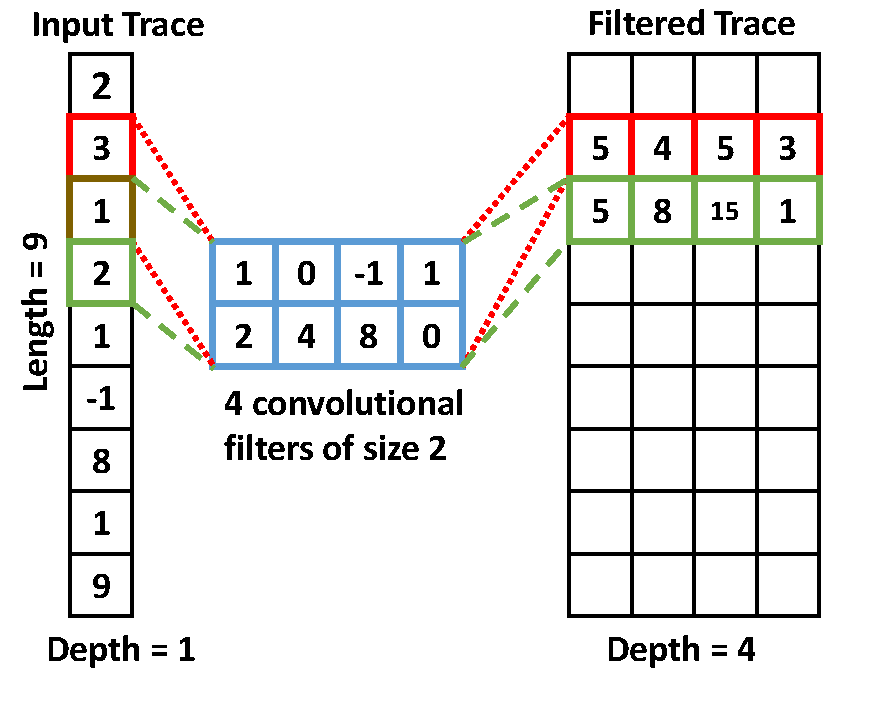
\includegraphics[width=.4\textwidth]{../Figures/CHES2017/conv_filt.pdf}}
%\subfigure[]{\label{fig:pool_layer}
%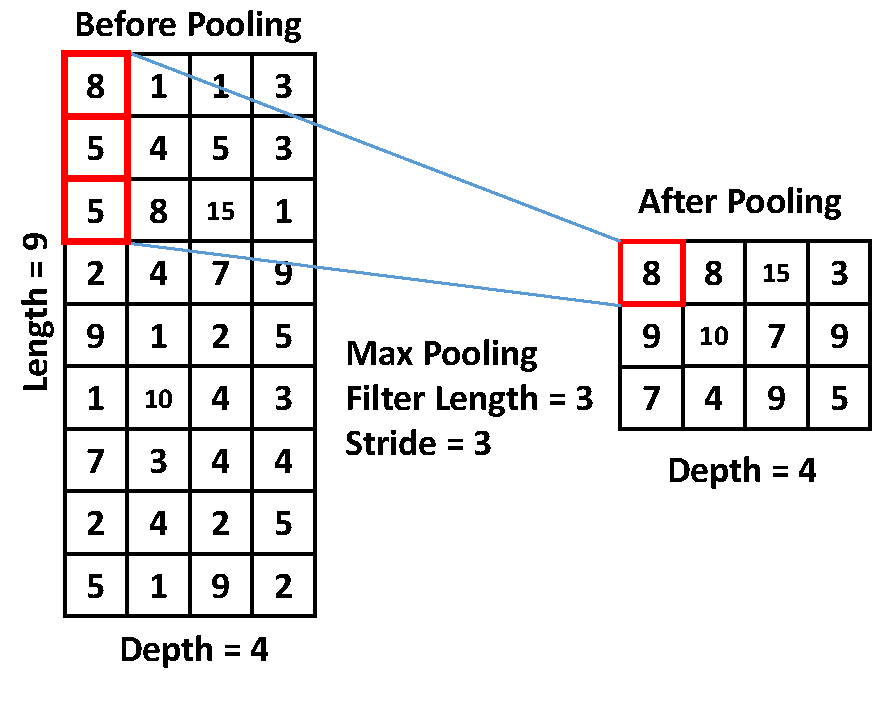
\includegraphics[width=.4\textwidth]{../Figures/CHES2017/max_pooling.pdf}}
%\caption{\subref{fig:conv_layer} Convolutional filtering: $W=2$, $V=4$, $\mathrm{stride}=1$. \subref{fig:pool_layer} Max-pooling layer: $W = \mathrm{stride} = 3$.}\label{fig:CNN_layers}
%\end{figure}

%\begin{figure}[t]
%\centering
%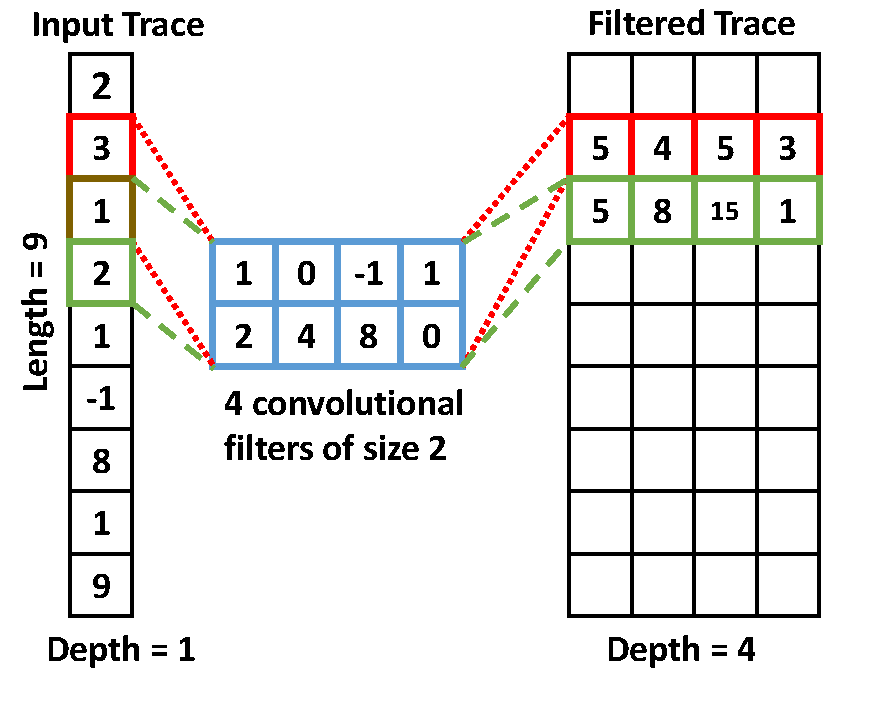
\includegraphics[width=.4\textwidth]{../Figures/CHES2017/conv_filt.pdf}
%\caption{Convolutional filtering: $W=2$, $V^{\prime}=4$, $\mathrm{stride}=1$. }\label{fig:conv_layer}
%\end{figure}
%

\begin{figure}
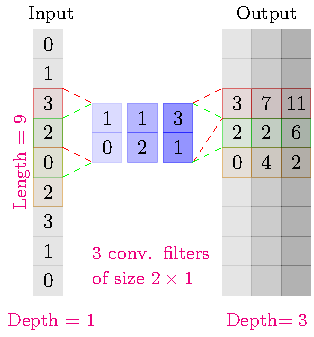
\includegraphics[scale=1, center]{../tikz_per_manuscritto/conv_filter_2_1.pdf} \\
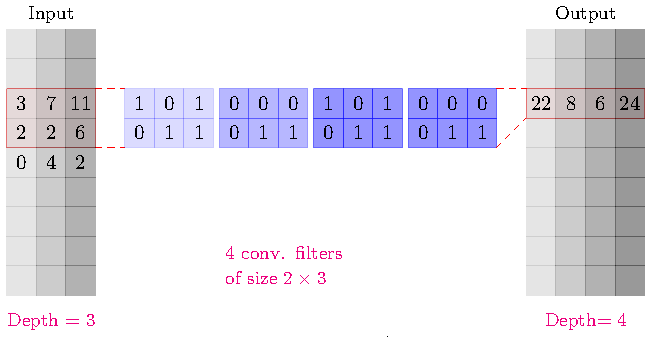
\includegraphics[scale=1, right]{../tikz_per_manuscritto/conv_filter_2_3.pdf} 

\caption[Convolutional layer.]{Two convolutional layers. Top: $W=2$, $V=1$, $n_{\text{filter}}=3$, $\mathrm{stride}=1$. Bottom: $W=2$, $V=3$, $n_{\text{filter}}=4$. }\label{fig:conv_layer}
\end{figure}

\begin{figure}[t]
\centering
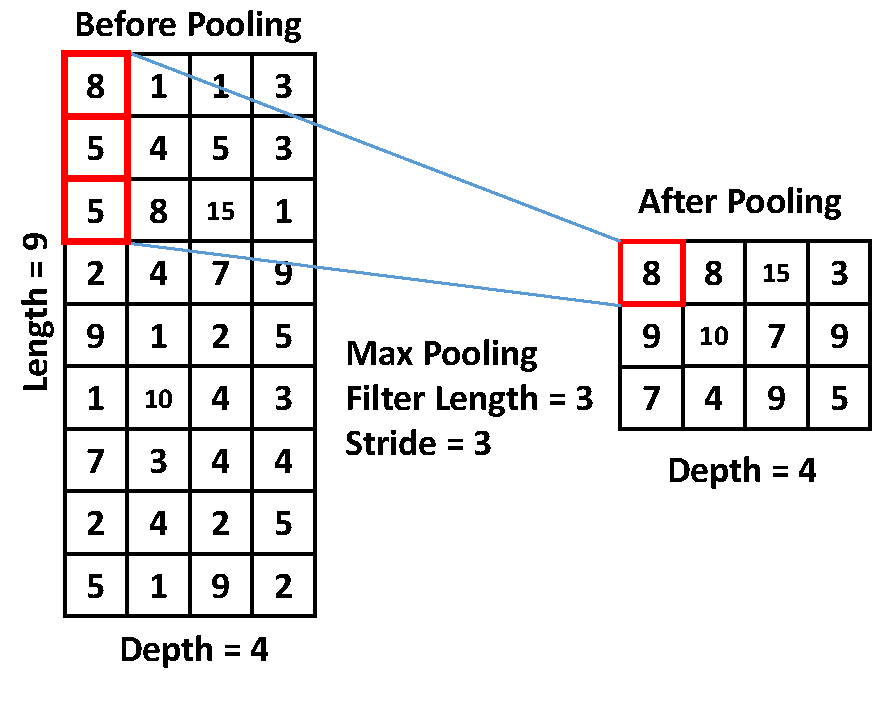
\includegraphics[width=.4\textwidth]{../Figures/CHES2017/max_pooling.pdf}
\caption[Max-pooling layer.]{Max-pooling layer: $W = \mathrm{stride} = 3$. }\label{fig:pool_layer}
\end{figure}

\paragraph*{Discussion}
The reason why a CONV always applies several filters (\ie $n_{\text{filter}}>1$) is
that we expect each filter to extract a different kind of feature from
the input. These extracted features are arranged
side-by-side over an additional data dimension, the so-called
\emph{depth}.\footnote{Ambiguity: Neural networks with more that one non-linear layer are called
\emph{Deep Neural Networks}, where the \emph{depth} corresponds to the number of
layers.} The hope is that during training, automatically, each filter specialises over the detection/recognition/modalisation of a different discriminant feature, and the collection of all discriminant features allows the last network layer concluding a successful classification.  As one goes along convolutional layers, higher-level abstraction
features are expected to be extracted.  The face recognition problem provides a simplified didactic example for this concept: we may think to some first layers' filters that specialise in detecting some local patterns of borders and surfaces. Then we may think to a deeper layer that compose such local features and modelise the angles of eyes' borders. the pupils, their color. Then some deeper layers may compose such feature and modelise  the whole eye, which is a more complex feature, and some deeper layers may compose eyes together with noses' features coming from other filters and, going on in this compositional process, modelise the whole face, and assign to it a very abstract feature, \ie the name of the person, which is the goal of the classification task. The fact that many natural data in the works have such a compositional flavour is one of the justifications inventors of CNNs provide to explain the success of such a technique.\footnote{See for example Yann LeCun's class available at \url{https://www.college-de-france.fr/site/yann-lecun/course-2016-02-12-14h30.htm}}  Actually, analysing and understanding the very first low-level features extracted by a self-trained CNN is a very hard task, and such an impossibility to explain from where discriminant features come out is, in my opinion, one of the characteristics of the DL domain that leads it to be kept unconsidered and disliked by a still quite large community of scientists. 

\paragraph*{Common architecture}
The main block of a CNN is a CONV layer $\gamma$ directly followed by an ACT layer $\sigma$. The former locally extracts information from the input thanks to its filters and the latter increases the capacity of the model thanks to its non-linearity. After some $ ( \sigma \circ \gamma)$  blocks, a POOL layer $\delta$ is usually added to reduce the number of neurons: $\delta \circ [ \sigma\circ \gamma]^{n_2} $. This new block is repeated in the neural network until obtaining an output of reasonable size. Then, some FCs are introduced in order to obtain a global result which depends on the entire input, and not only on local features. To sum-up, a common convolutional network can be characterized by the following formula:\footnote{where each layer of the same type appearing in the composition is not to be intended as exactly the same function (\eg with same input/output dimensions), but as a function of the same form.} 
\begin{equation}\label{equ:CCN}
  \softmax \circ [\lambda]^{n_1} \circ[\delta \circ [\sigma \circ \gamma  ]^{n_2} ]^{n_3}  .
\end{equation}

 Layer by layer the network increases the spatial depth through convolution filters, adds non-linearity through activation functions and reduces the spatial (or temporal, in the side-channel traces case) size through pooling layers. Once a deep and narrow representation has been obtained, one or more FC layers are connected to it, followed by a softmax function. An example of CNN architecture is represented in Fig.~\ref{fig:archi_conv}. 
\begin{figure}[h]
\centering
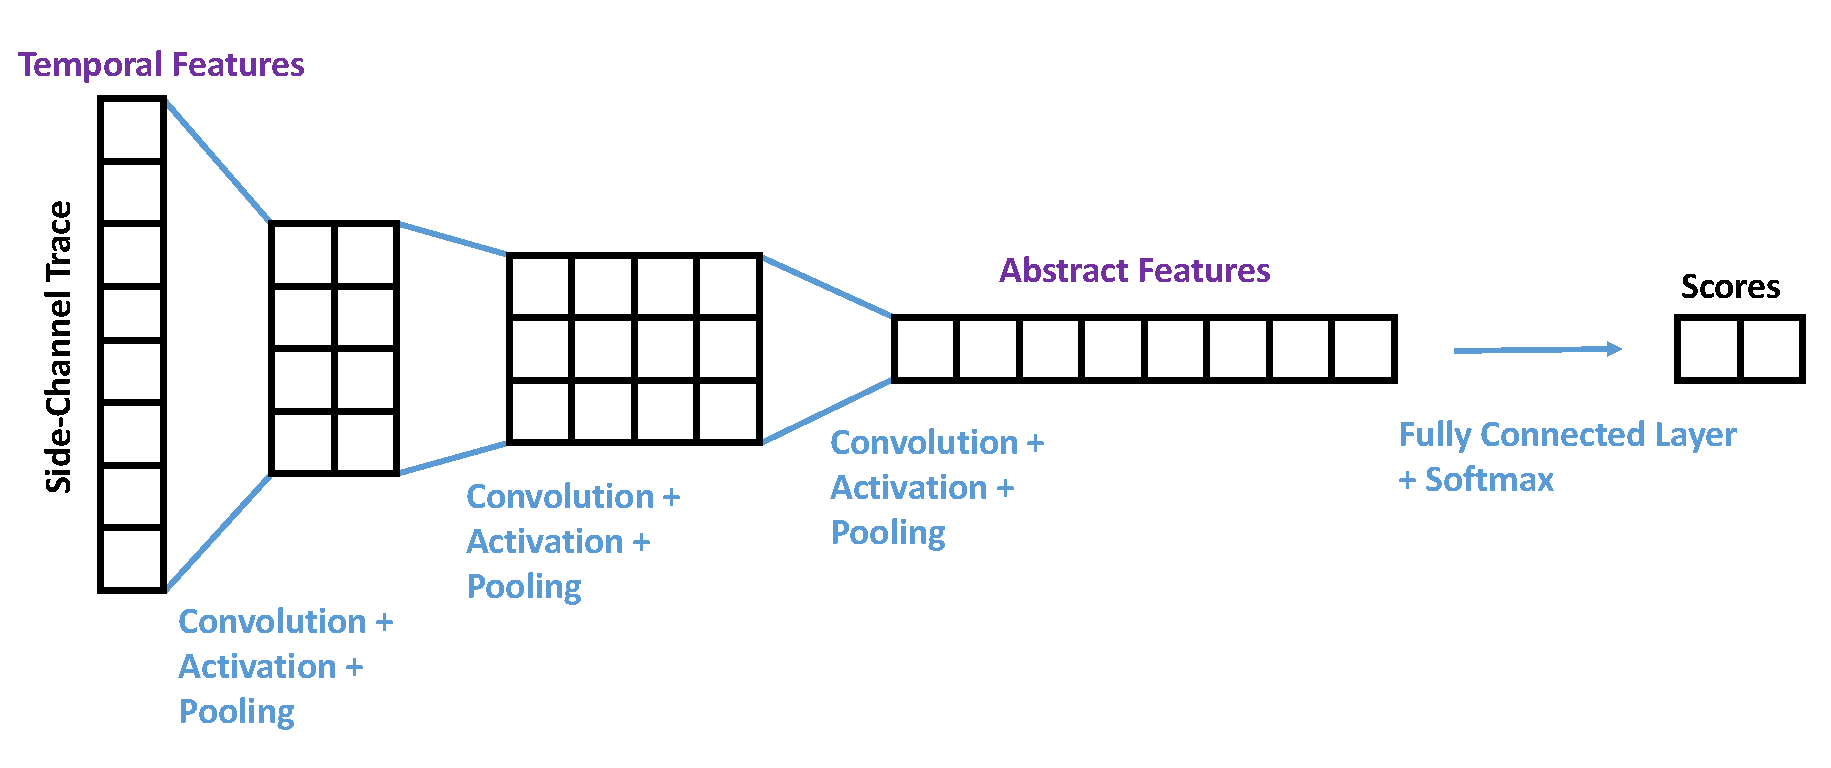
\includegraphics[width=\textwidth]{../Figures/CHES2017/convnet_arch.pdf}
\caption{Common CNN architecture.}
\label{fig:archi_conv}
\end{figure} 



\section{Data Augmentation}\label{sec:DA}
As explained in Sec.~\ref{sec:overfitting}, ML models are prone to overfitting, especially when their capacity (see Sec.~\ref{sec:overfitting}) is very high, as it is often the case with deep networks. Thus, it is sometimes necessary to deal with the overfitting phenomenon, by applying some regularization techniques. As we will see in Secs. \ref{sec:soft} and \ref{sec:hard} this will be the case in our experiments: indeed we will propose a quite deep CNN architecture,  flexible enough to successfully manage the misalignment problems, but trained over some relatively small training sets. This fact, combined with the high capacity of our CNN architecture, implies that the model will \emph{learn by heart} each element of the training set, without catching the truly discriminant features of the traces.\\

Instead of applying a proper regularization techniques, we choose to concentrate priorly on the Data Augmentation strategy \cite{simard2003best}, mainly for two reasons. First, it is a common practice in side-channel context to increase the number of acquisitions to counteract the misalignment effect. In other terms, misalignment may provoke a \textquotedbl lack of data\textquotedbl phenomenon on adversary's side. In the ML domain, such a lack is classically addressed thanks to the DA technique, and its benefits are widely proved. For example, many image recognition competition winners made use of such a technique (\eg the winner of ILSVRC-2012 \cite{KSH12}). Second, the DA is controllable, meaning that the deformations applied to the data are chosen, thus fully characterized. It is therefore possible to fully determine the addition of complexity induced to the classification problem. In our opinion, other techniques add constraints to the problem in a more implicit and uncontrollable way, \eg the dropout \cite{HSKSS12}  or the $\ell_2$-norm regularization \cite{christopher2006pattern}.\\

Data augmentation consists in artificially generating new training traces by deforming those previously acquired. The deformation is done by the application of transformations that preserve the  label information (\ie the value of the handled sensitive variable in our context). We choose two kinds of deformations, that we denote by \emph{Shifting} and \emph{Add-Remove}. 

\paragraph*{Shifting Deformation ($\mathrm{SH}_{T^\star}$)} It simulates a random delay effect of maximal amplitude $T^\star$, by randomly selecting  a shifting window of the acquired trace, as shown in Fig. \ref{fig:SH}. Let $\traceLength$ denote the original size of the traces. We fix the size of the input layer of our CNN to $\traceLength^\prime = \traceLength - T^\star$. Then the technique $\mathrm{SH}_{T^\star}$  consists (1) in drawing a uniform random $t \in[0,T^\star]$, and (2) in selecting the $\traceLength^\prime$-sized window starting from the $t$-th point. For our study, we will compare the $\mathrm{SH}_T$ technique for different values $T \leq T^\star$, without changing the architecture of the CNN (in particular the input size $\traceLength^\prime$). Notably, $T \lneq T^\star$ implies that $T^\star-T$ time samples will never have the chance to be selected. As we suppose that the information is localized in the central part of the traces, we choose to center the shifting windows, discarding the heads and the tails of the traces (corresponding to the first and the last $\frac{T^\star-T}{2}$ points). 

\paragraph*{Add-Remove Deformation ($\mathrm{AR}$)}  It simulates a clock jitter effect (Fig. \ref{fig:AR}). We will denote by $\mathrm{AR}_R$ the operation that consists in two steps:
\begin{itemize}
\item[(1)] in inserting $R$ time samples, whose positions are chosen uniformly at random and whose values are the arithmetic mean between the previous time sample and the following one,
\item[(2)] in suppressing $R$ time samples, chosen uniformly at random.\\
\end{itemize}

The two deformations can be composed: we will denote by $\mathrm{SH}_T\mathrm{AR}_R$ the application of a $\mathrm{SH}_T$ followed by a $\mathrm{AR}_R$.

%
%\begin{figure}[t]
%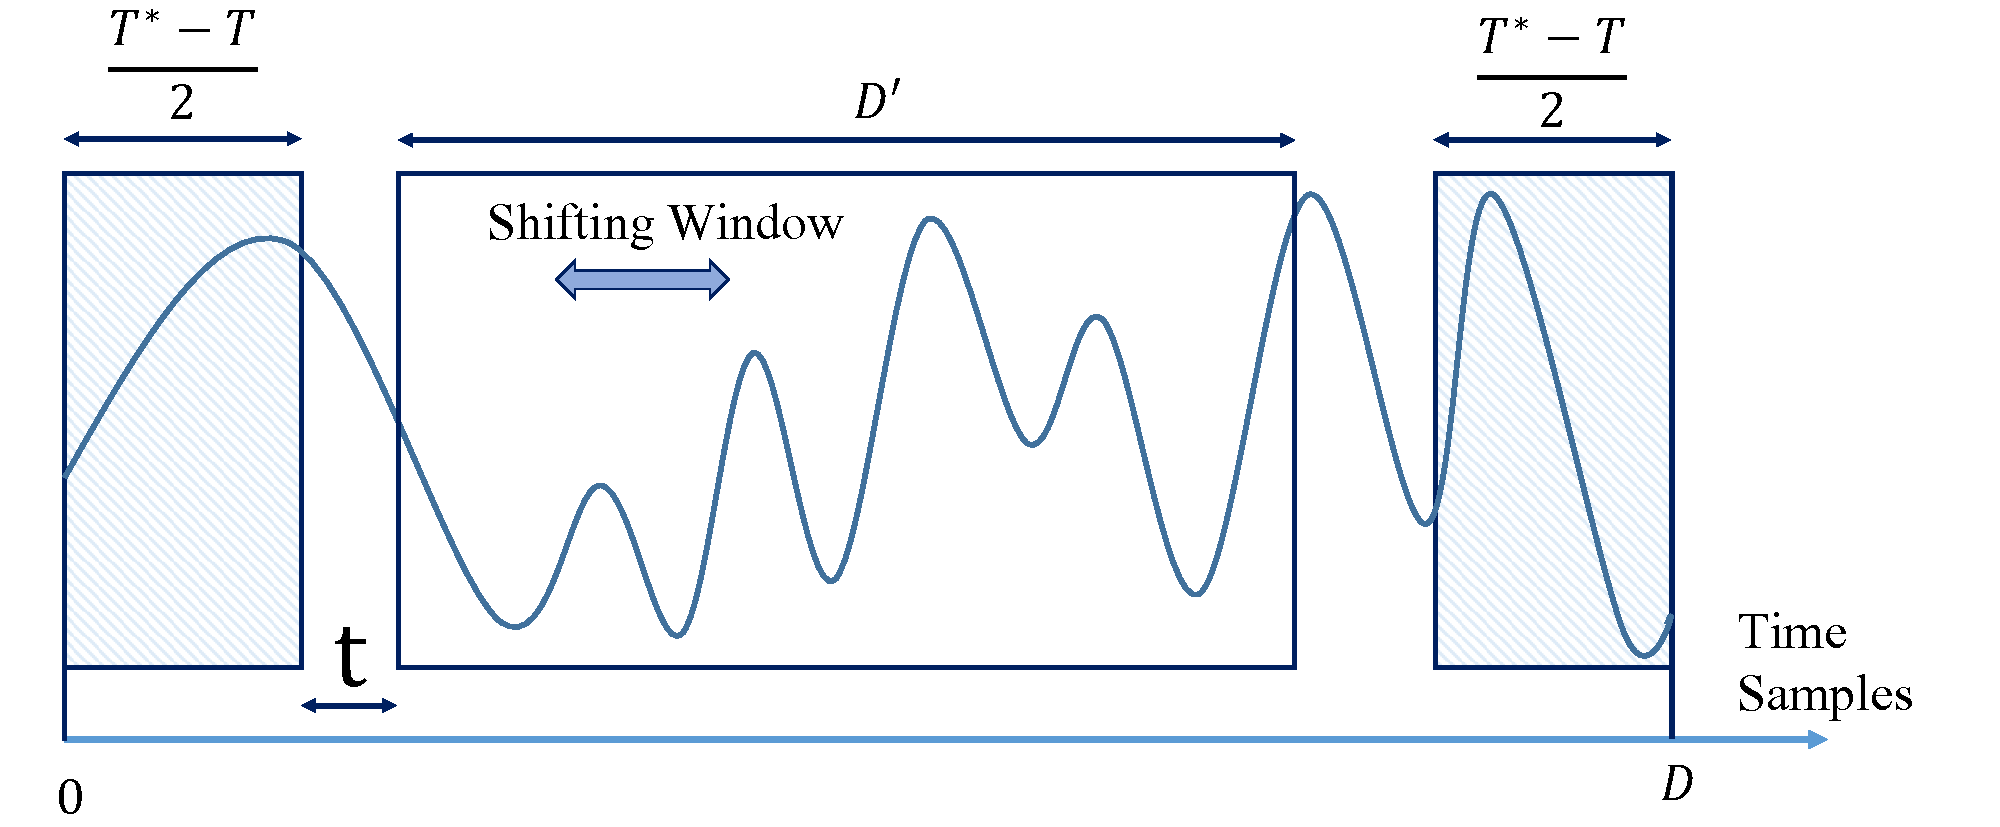
\includegraphics[width=.5\textwidth, height=0.13\textheight]{../Figures/CHES2017/Shifting_window.pdf}
%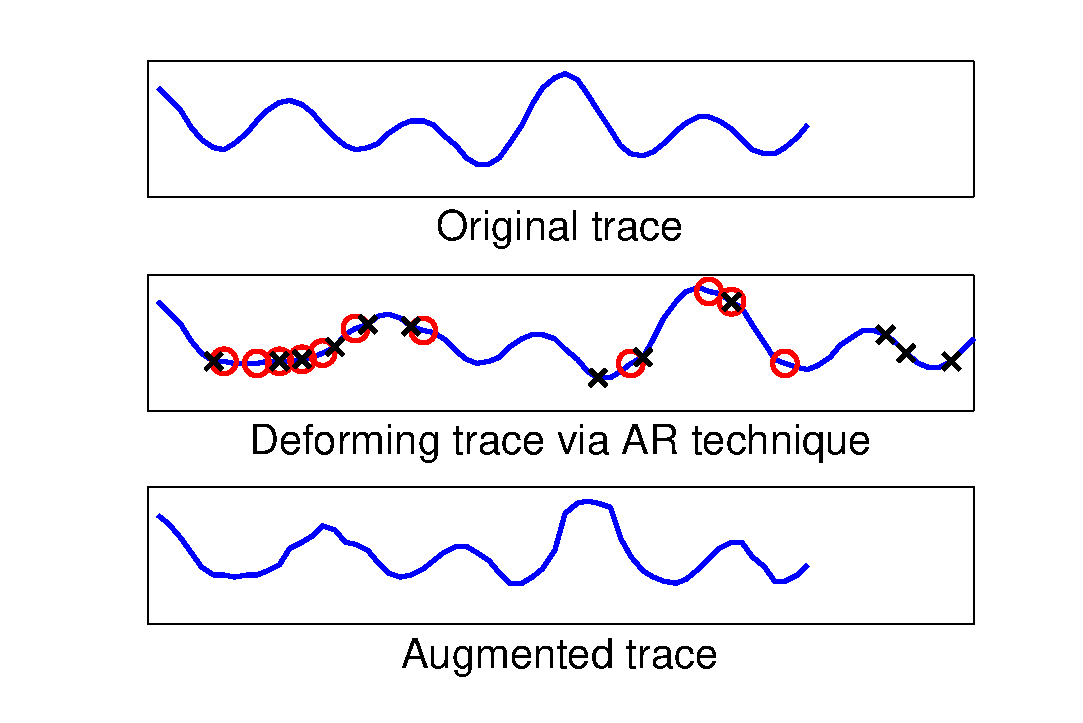
\includegraphics[width=.5\textwidth, height=0.13\textheight]{../Figures/CHES2017/AR_example.pdf}
%\caption{Left: Shifting technique for DA. Right: Add-Remove technique for DA (added points marked by red circles, removed points marked by black crosses).}\label{fig:DA}
%\end{figure}


\begin{figure}[t]
\centering
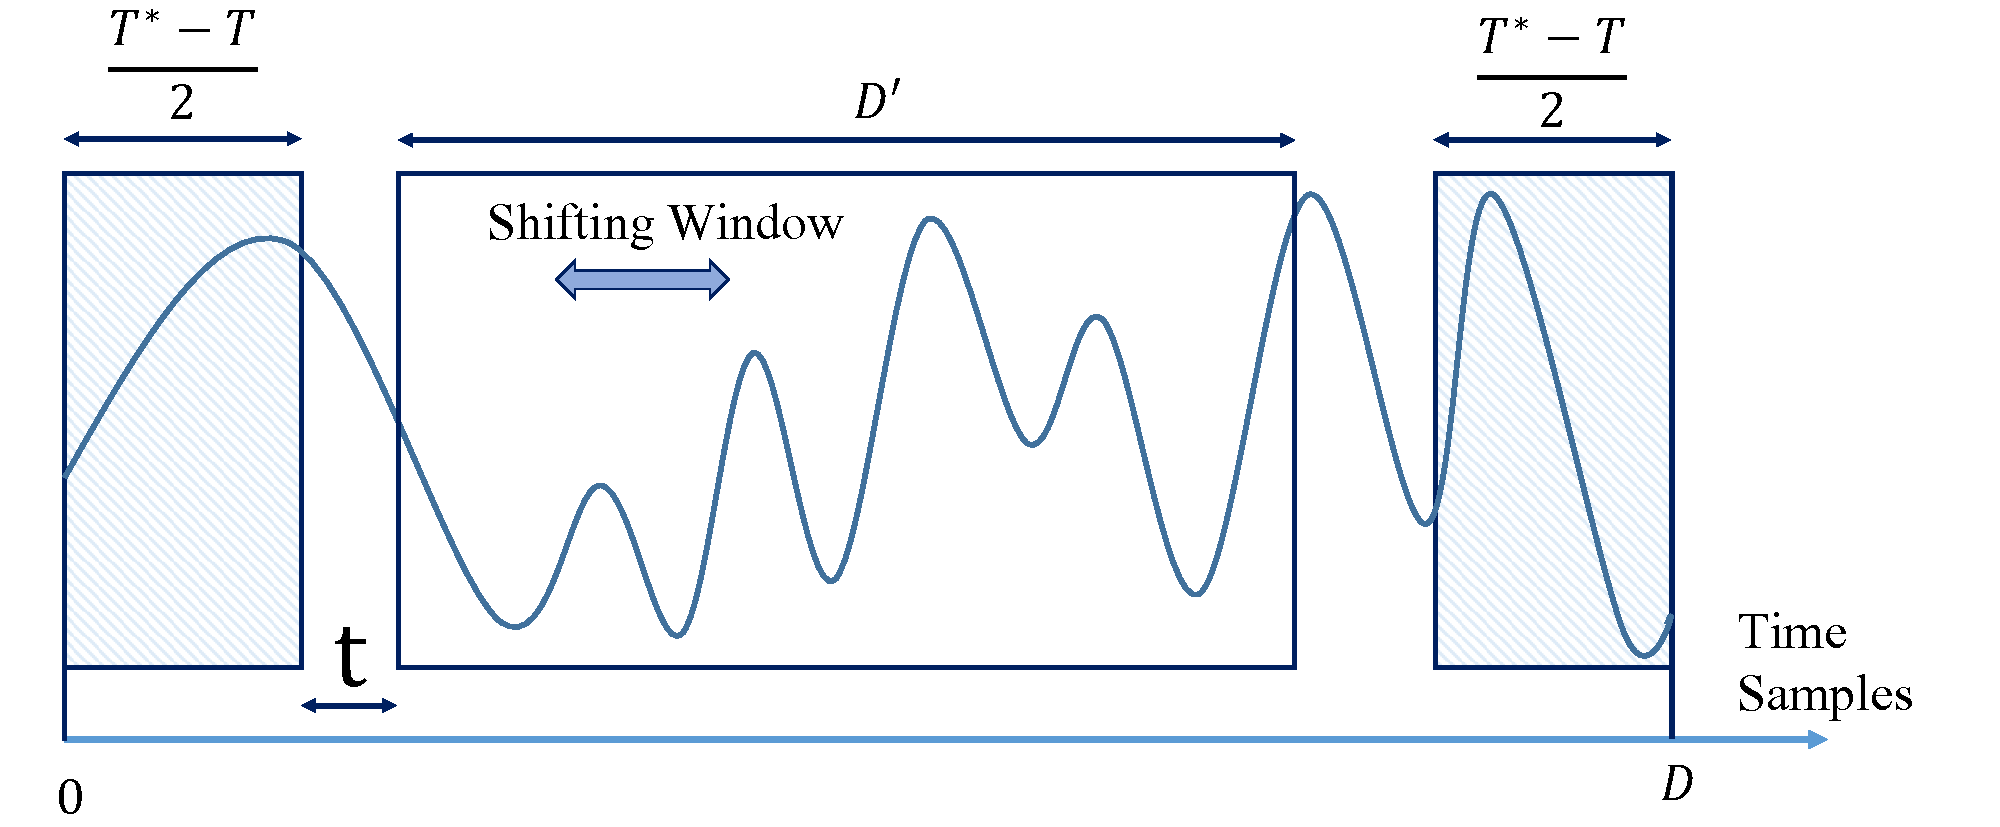
\includegraphics[width=.5\textwidth]{../Figures/CHES2017/Shifting_window.pdf}
\caption{Shifting technique for DA.}\label{fig:SH}
\end{figure}

\begin{figure}[t]
\centering
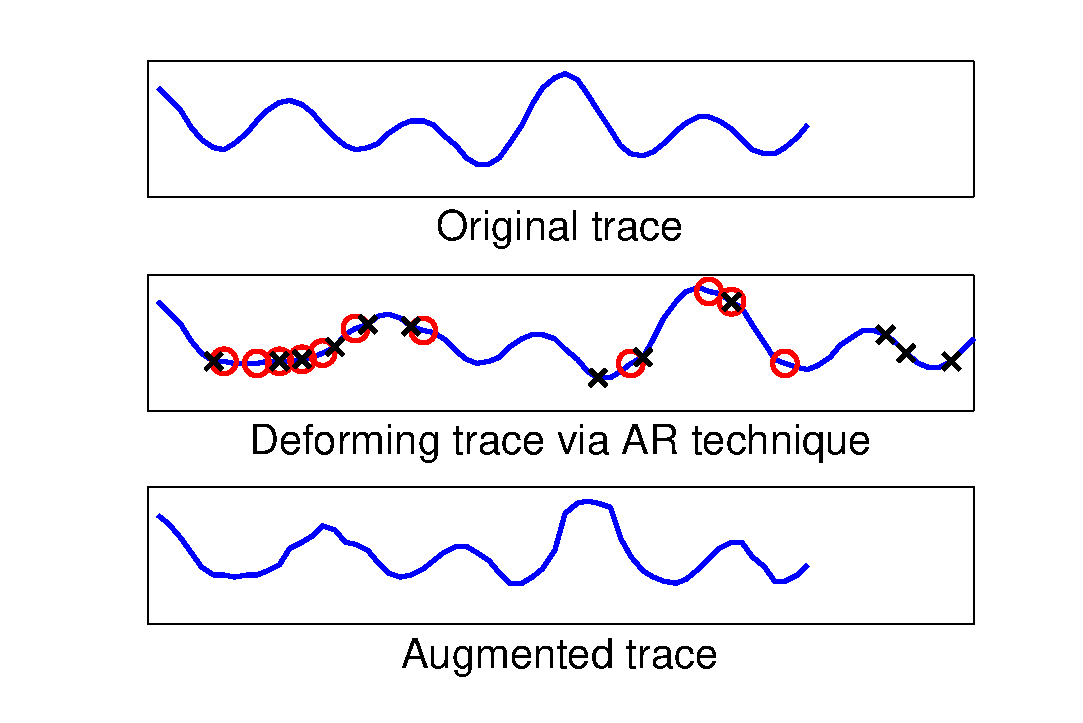
\includegraphics[width=.5\textwidth]{../Figures/CHES2017/AR_example.pdf}
\caption[Add-Remove technique for DA.]{Add-Remove technique for DA (added points marked by red circles, removed points marked by black crosses).}\label{fig:AR}
\end{figure}

\paragraph*{Discussion}
The deformations we propose as Data Augmentation techniques are inspired by the way we modelise the countermeasures' effects. Actually, we propose to turn the misalignment problem into a virtue, enlarging the profiling trace set \via a random shift of the acquired traces and the AR distortion that together simulate a clock jitter effect. Paradoxically, instead of trying to realign the traces, we propose to further misalign them (a much easier task!). In real-case secure devices evaluation contexts, the acquisition campaign may sometimes represent a bottleneck in terms of time. Further proposals and analyses of  DA techniques, maybe inspired by other forms of noise present in side-channel acquisitions, might be interesting tracks for future researches. Actually, the idea of applying DA in profiling side-channel context appeared independently from our work, in another publication in 2017 \cite{pu2017trace}, under the name of \emph{Trace Augmentation}. In this paper, the augmentation is obtained with a shifting equivalent to our SH deformation, and it is applied as preliminary step for the profiling phase of a Gaussian TA. The authors' goal is to make Gaussian templates more robust to the discrepancy between profiling acquisitions and attack ones. Surprisingly, in the paper, authors observe that this augmentation provides benefits to the attack routine both in case where some discrepancies are present, and in the ideal case. Data Augmentation seems thus to be a good practice independently of the presence or not of specific countermeasures, nor the exploitation or not of DL techniques.



\section{Experiments against Software Countermeasures}

\begin{figure}
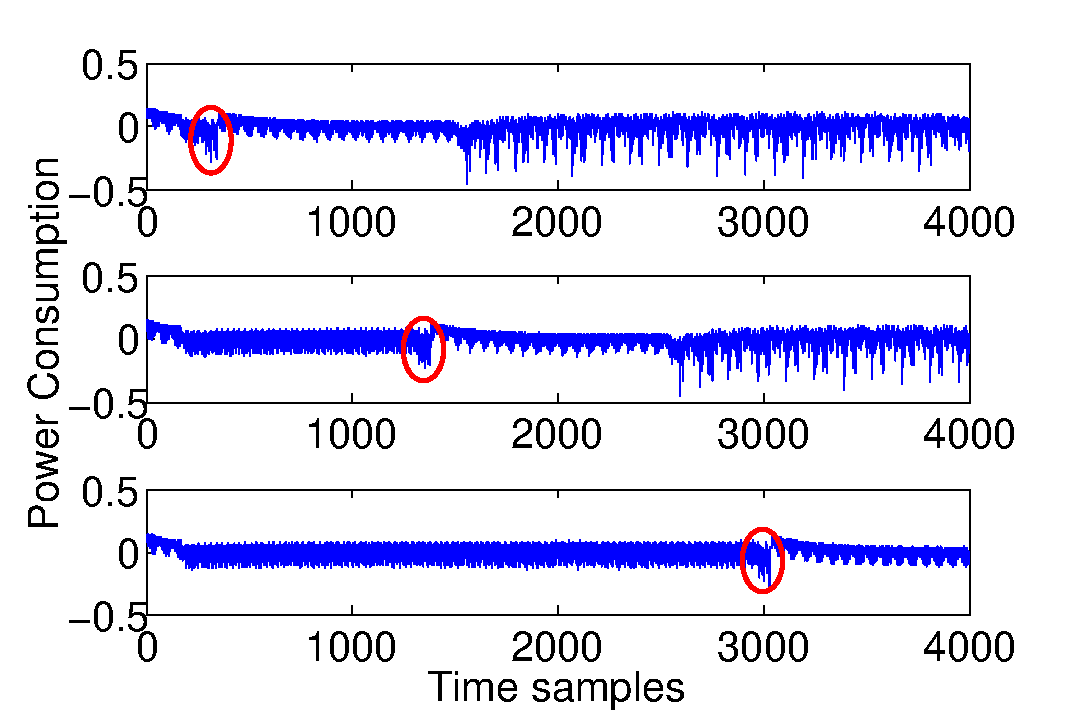
\includegraphics[width=.5\textwidth]{../Figures/CHES2017/CW_shift_traces.pdf} 
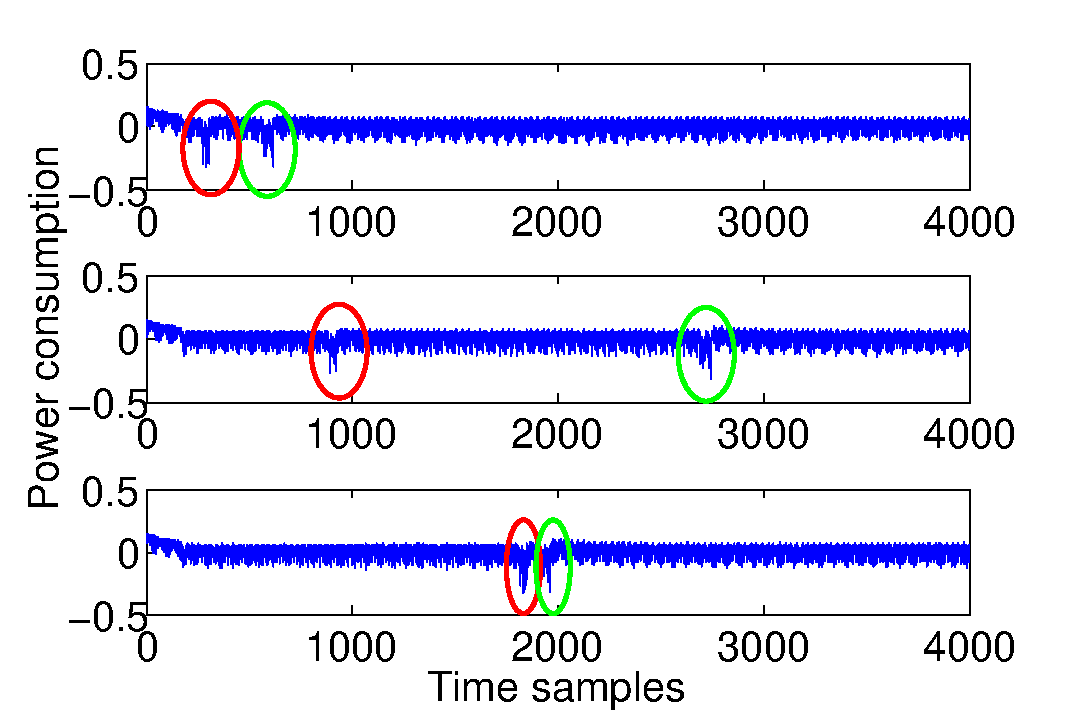
\includegraphics[width=.5\textwidth]{../Figures/CHES2017/CW_double_shift_traces.pdf} 
\caption[Leakages hidden by Random Delay Interruption.]{Left: one leakage protected by single uniform RDI. Right: two leaking operations protected by multiple uniform RDI.}\label{fig:CW_shift_traces}
\end{figure}

In this section we present two preliminary  experiments, performed in order to validate the shift-invariance claimed by the CNN architecture, recalled in Sec.~\ref{sec:CNN}. In the first one, a single leaking operation was observed through the side-channel acquisitions, shifted in time by the insertion of a random number of dummy operations. We will refer to such a countermeasure as Random Delay Interrupt (RDI).  In the second one we targeted two leaking operations each delayed by RDI. We remark that this kind of countermeasure is nowadays considered defeated, \eg thanks to resynchronisation by \emph{cross-correlation} \cite{nagashima2007dpa}. In this sense, the experiment we present in this section is not expected to be representative of real application cases. The complexity of the state-of-the-art resynchronisation techniques strongly depends on the variability of the shift. When the latter variability is low, \ie when attacks are judged to be applicable, multiple random delays are recommended. It has even been proposed to adapt the probabilistic distributions of the random delays to achieve good compromises between the countermeasure efficiency and the chip performance overhead \cite{coron2009efficient,coron2010analysis}. Attacks have already been shown even against this multiple-RDI kind of countermeasures, \eg \cite{durvaux2012efficient}. The latter attack exploits some Gaussian templates to classify the leakage of each instruction; the classification scores are used to feed a Hidden Markov Model (HMM) that describes the complete chip execution, and the Viterbi algorithm is applied to find the most probable sequence of states for the HMM and to remove the random delays. We remark that this HMM-based attack exploits Gaussian templates to feed the HMM model, and the accuracy of such templates is affected by other misalignment reasons, \eg clock jitter. We believe that our  CNN approach proposal for operation classification, is a valuable alternative to  the Gaussian template one, and might even provide benefits to the HMM performances, by \eg improving the robustness of the attack in presence of both RDI and jitter-based countermeasures. This robustness w.r.t. of misalignment caused by the clock jitter will be analysed in Sec. \ref{sec:hard}.

\subsection{One Leaking Operation}\label{sec:soft}
For this experiment, we implemented, on an Atmega328P microprocessor, a uniform RDI \cite{tunstall2007efficient} to protect the leakage produced by a single target operation. Our RDI simply consists in a loop of  $r$ \emph{nop} instructions, with $r$  drawn uniformly in $[0,127]$. Some acquired traces are reported in the left side of Fig. \ref{fig:CW_shift_traces}, the target peak being highlighted with a red ellipse. They are composed of $3,996$ time samples, corresponding to an access to the AES-Sbox look-up table stored in NVM. For the training, we acquired only $1,000$ traces and 700 further traces were acquired as validation data. Our CNN has been trained to classify the traces according to the Hamming weight of the Sbox output; namely, our labels are the nine values taken by $\sensRandVar = \HW(\Sbox(P\oplus \keyRandVar))$. This choice has been done to let each class contain more than only a few (i.e. about $1,000/256$) training traces.
For Atmega328P devices, the Hamming weight is known to be particularly relevant to model the leakage occurring during register writing (see for example Chapters~\ref{ChapterLinear} and \ref{ChapterKernel} or \cite{BelaidCFGKP15}). Since $\sensRandVar$ is assumed to take nine values and the position of the leakage depends on a random $r$ ranging over 128 values, it is clear that the $1,000$ training traces do not encompass the full $9 \times 128=1,152$ possible combinations $(z,r)\in [0,8]\times[0,127]$. We undersized the training set by purpose, in order to establish whether the CNN technique, equipped with DA, is able to catch the meaningful shift-invariant features without having been provided with all the possible observations.\\


\begin{figure}[t]
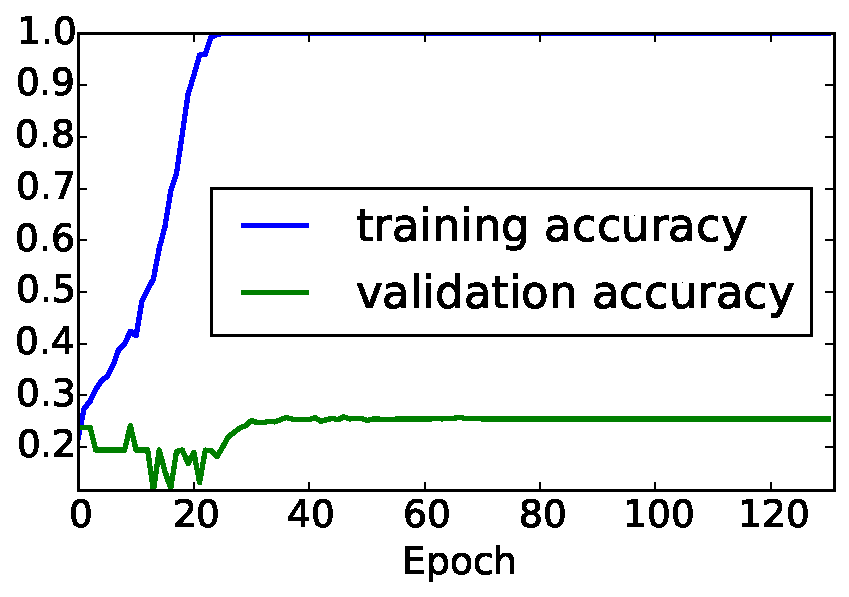
\includegraphics[width=.30\textwidth]{../Figures/CHES2017/DAshift0_2000traces_9classes_sgd/acc_DAshift0_2000traces_9classes_sgd.pdf} 
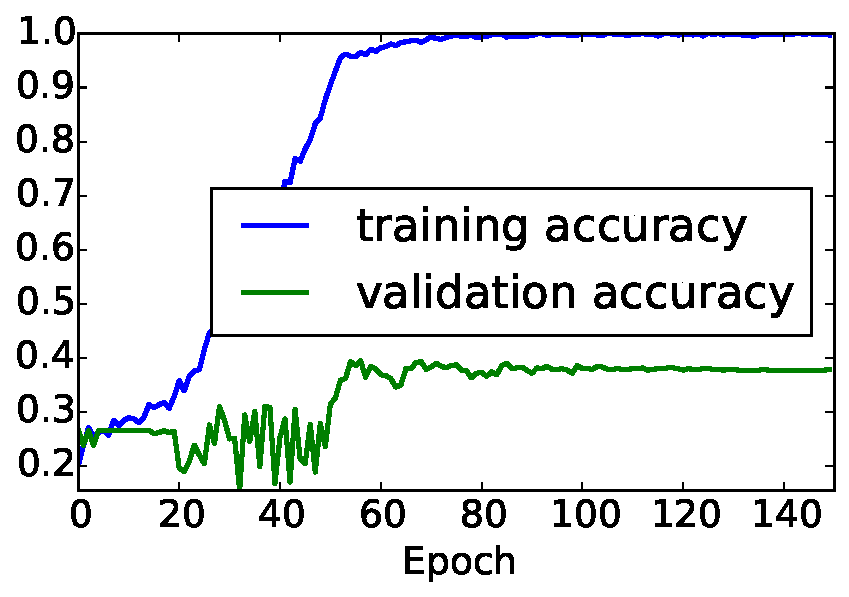
\includegraphics[width=.30\textwidth]{../Figures/CHES2017/DAshift100_2000traces_9classes_sgd/acc_DAshift100_2000traces_9classes_sgd.pdf} 
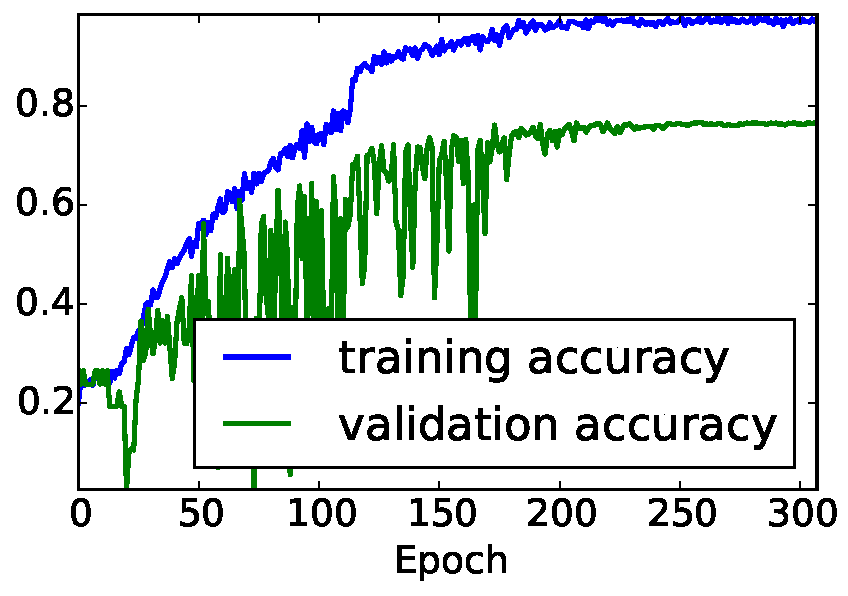
\includegraphics[width=.30\textwidth]{../Figures/CHES2017/DAshift500_2000traces_9classes_sgd/acc_DAshift500_2000traces_9classes_sgd.pdf}\\ 
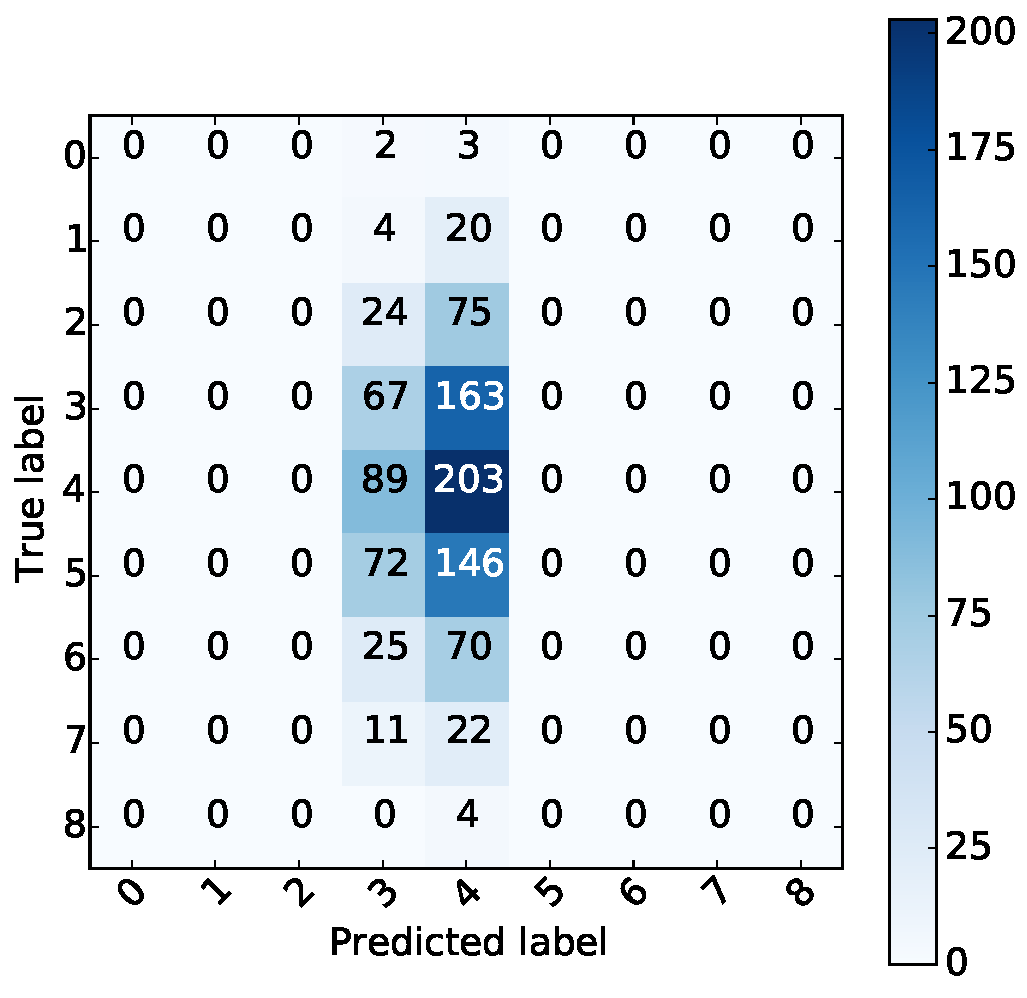
\includegraphics[width=.30\textwidth]{../Figures/CHES2017/DAshift0_2000traces_9classes_sgd/CM_DAshift0_2000traces_9classes_sgd.pdf} 
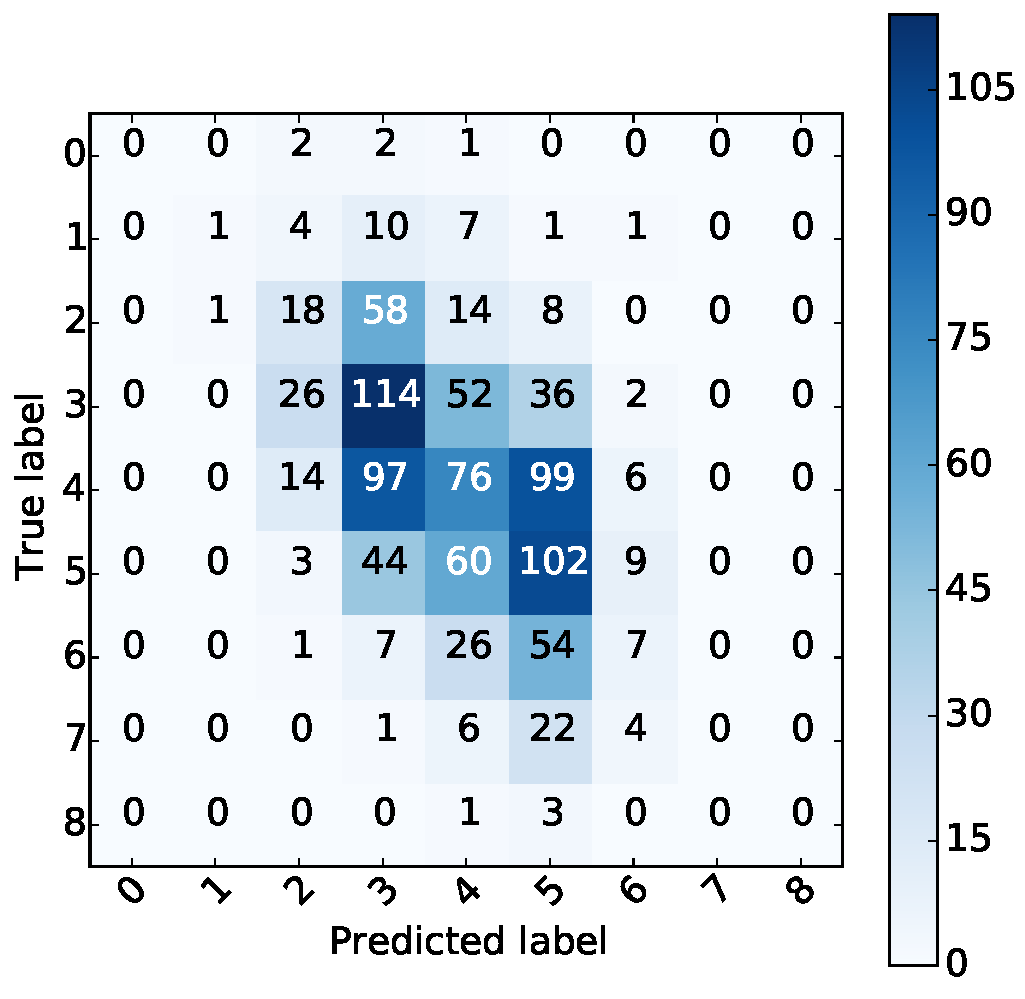
\includegraphics[width=.30\textwidth]{../Figures/CHES2017/DAshift100_2000traces_9classes_sgd/CM_DAshift100_2000traces_9classes_sgd.pdf} 
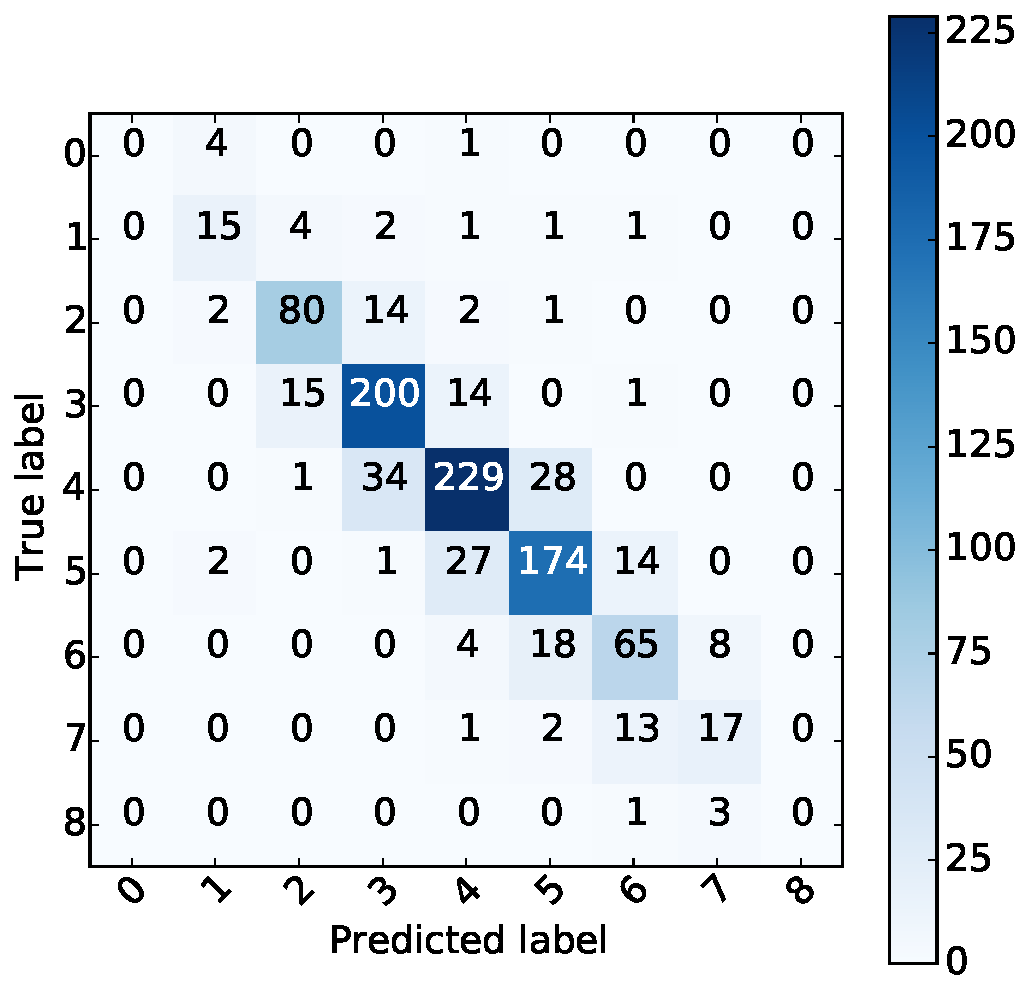
\includegraphics[width=.30\textwidth]{../Figures/CHES2017/DAshift500_2000traces_9classes_sgd/CM_DAshift500_2000traces_9classes_sgd.pdf}
\caption[Software misalignment: accuracies vs epochs and confusion matrices obtained with our CNN for different DA techniques.]{One leakage protected via uniform RDI: accuracies vs epochs and confusion matrices obtained with our CNN for different DA techniques. From left to right: $\mathrm{SH}_0$, $\mathrm{SH}_{100}$, $\mathrm{SH}_{500}$. }\label{fig:CW_shift_history}
\end{figure}

For the training of our CNN, we applied the $SH_T$ data augmentation, selecting $T^\star = 500$ and $T \in \{ 0,100, T^\star\}$; this implies that the input dimension of our CNN is reduced to $3,496$. Our implementation is based on Keras library \cite{keras} (version 1.2.1), and we run the trainings over an ordinary computer equipped with a gamers market GPU, a GeForce GTS 450. For the CNN architecture, we chose the following structure: 
\begin{equation}\label{eq:archi}
  \softmax \circ [\lambda]^1 \circ[\delta \circ [\sigma \circ \gamma  ]^1 ]^4,   
\end{equation}
\emph{i.e.} \eqref{equ:CCN} with $n_1 = n_2 = 1$ and $n_3 = 4$.
To accelerate the training we applied a technique proposed in 2015 \cite{batch_norm}, consisting in the  introduction of a so-called \emph{Batch Normalization} layer \cite{batch_norm} after each pooling $\delta$. The network transforms the $3,496 \times 1$ inputs in a $1 \times 256$ list of abstract features, before entering the last FC layer $\lambda:\mathbb{R}^{256}\rightarrow \mathbb{R}^9$. Even if the ReLU activation function \cite{nair2010rectified} is classically recommended for many applications in literature (see Sec.~\ref{sec:MLP}), we obtained in most cases better results using the hyperbolic tangent, defined as:
\begin{equation}
\mathrm{tanh}(x) = \frac{e^x-e^{-x}}{e^x+e^{-x}} \mbox{ .}
\end{equation}
We trained our CNN by batches of size $32$.  In total the network contained $869,341$ trainable weights. The training and validation accuracies achieved after each epoch are depicted in Fig.\ref{fig:CW_shift_history} together with the confusion matrices that we obtained from the test set. Applying the early-stopping principle recalled in Sec.~\ref{sec:training},  we automatically stopped the training after $120$ epochs without decrement of the loss function evaluated over the validation set, and kept as final trained model the one that showed the minimal value for the loss function evaluation. Concerning the learning rate (see Sec.~\ref{sec:training}), we fixed the beginning one to $0.01$ and reduced it multiplying it by a factor of $\sqrt{0.1}$ after $5$ epochs without validation loss decrement.


\begin{table}[t]
\centering
\caption[Results of our CNN, for different DA techniques, in presence of an uniform RDI countermeasure protecting.]{Results of our CNN, for different DA techniques, in presence of an uniform RDI countermeasure protecting. For each technique, $4$ values are given: in position $a$ the maximal training accuracy, in position $b$ the maximal validation accuracy, in position $c$ the test accuracy, in position $d$ the value of $N^\star$ (see Sec.~\ref{sec:performances_NN} for definitions).}
\label{tab:res_CW_shift}
\begin{tabular}{|c|c|c|c|c|c|c|c|}
\hline
\multicolumn{2}{|c|}{} & \multicolumn{2}{c|}{$\mathrm{SH}_{0}$}                                    & \multicolumn{2}{c|}{$\mathrm{SH}_{100}$} & \multicolumn{2}{c|}{$\mathrm{SH}_{500}$} \\ \hline
$a$        & $b$       & \cellcolor[HTML]{EFEFEF}100\%  & \cellcolor[HTML]{EFEFEF}25.9\%           & 100\%               & 39.4\%             & \textbf{98.4\%}     & \textbf{76.7\%}    \\ \hline
$c$        & $d$       & \cellcolor[HTML]{EFEFEF}27.0\% & \cellcolor[HTML]{EFEFEF}\textgreater1000 & 31.8\%              & 101                & \textbf{78.0\%}     & \textbf{7}         \\ \hline
\end{tabular}
\end{table}

Table \ref{tab:res_CW_shift} summarizes the obtained results.  For each trained model we can compare the maximal training accuracy achieved during the training with the maximal validation accuracy, defined in Sec.~\ref{sec:performances_NN}.  This comparison gives an insight about the risk of overfitting for the training.\footnote{The validation accuracies are estimated over a 700-sized set, while the test accuracies are estimated over $100,000$ traces. Thus the latter estimation is more accurate, and we recall that the test accuracy is to be considered as the final CNN classification performance.} Case $\mathrm{SH}_0$ corresponds to a training performed without DA technique. When no DA is applied, the overfitting effect is dramatic: the training set is $100\%$-successfully classified after about $22$ epochs, while the test accuracy only achieves $27\%$. The $27\%$ is around the rate of uniformly distributed bytes showing an Hamming weight of $4$.\footnote{We recall that the Hamming weight of uniformly distributed data follows a binomial law with coefficients $(8,0.5)$.} Looking at the corresponding confusion matrix we remark that the CNN training has been biased by the binomial distribution of the training data, and almost always predicts the class $4$. This essentially means that no discriminative feature has been learned in this case, which is confirmed by the fact that the trained model leads to an unsuccessful attack ($N^\star>1,000$). Remarkably, the more artificial shifting is added by the DA, the more the overfitting effect is attenuated; for $SH_T$ with \eg $T=500$ the training set is never completely learnt and the test accuracy achieves $78\%$, leading to a guessing entropy of 1 with only $N^{\star}=7$ traces. \\

These results confirm that our CNN model is able to characterize a wide range of points in a way that is robust to RDI. 

\subsection{Two Leaking Operations}
Here we study whether our CNN classifier suffers from the presence of multiple leaking operations with the same power consumption pattern. This situation occurs for instance any time the same operation is repeated several successive times over different pieces of data (\eg the SubByte operation for a software AES implementation is often performed by 16 successive look-up table accesses). To start our study we performed the same experiments as in Sec.~\ref{sec:soft} over a second traces set, where two look-up table accesses leak, each preceded by a random delay. Some examples of this second traces set are given in the right side of Fig.~\ref{fig:CW_shift_traces}, where the two leaking operations being highlighted by red and green ellipses. We trained the same CNN as in Sec.~\ref{sec:soft}, once to classify the first leakage, and a second time to classify the second leakage, applying $\mathrm{SH}_{500}$ as DA technique. Results are given in Table~\ref{tab:label}. They show that even if the CNN transforms spatial (or temporal) information into abstract discriminative features, it still holds an ordering notion: indeed if no ordering notion would have been held, the CNN could no way discriminate the first peak from the second one. 


\begin{table}[]
\centering
\caption[Results of our CNN in presence of uniform RDI protecting two leaking operations.]{Results of our CNN in presence of uniform RDI protecting two leaking operations. See the caption of Table~\ref{tab:res_CW_shift} for a legend.}
\label{tab:label}
\begin{tabular}{|c|c|c|c|c|c|}
\hline
\multicolumn{2}{|c|}{} & \multicolumn{2}{c|}{First operation} & \multicolumn{2}{c|}{Second operation} \\ \hline
$a$        & $b$       & 95.2\%            & 79.7\%           & 96.8\%            & 81.0\%            \\ \hline
$c$        & $d$       & 76.8\%            & 7                & 82.5\%            & 6                 \\ \hline
\end{tabular}
\end{table}




%----------------------------------------------------------------------------------------
%	SECTION 6
%----------------------------------------------------------------------------------------


\section{Experiments against Artificial Hardware Countermeasures}\label{sec:hard}

A classical hardware countermeasure against side-channel attacks consists in introducing instability in the clock. This implies the cumulation of a deforming effect that affects each single acquired clock cycle, and provokes traces misalignment on the adversary side. Indeed, since clock cycles do not have the same duration, they are sampled during the attack by a varying number of time samples. As a consequence, a simple translation of the acquisitions is not sufficient in this case to align with respect to an identified clock cycle. Several realignment techniques are available to manage this kind of deformations, \eg \cite{van2011improving}. In this context, our goal is to show that  we can get rid of the realignment pre-processing, letting the CNN deep structure take it in charge implicitly. 

\subsection{Performances over Artificial Augmented Clock Jitter}\label{sec:artificial}
In this section we present the results that we obtained over two datasets named \emph{DS\_low\_jitter} and \emph{DS\_high\_jitter}. Each one contains $10,000$ labelled traces, used for the training phase (more precisely, $9,000$ are used for the training, and $1,000$ for the validation), and $100,000$ attack traces. The traces are composed of $1,860$ time samples. The two datasets have been obtained by artificially adding a simulated jitter effect over some synchronised original traces. The original traces were measured on the same Atmega328P microprocessor used in the previous section. We verified that they originally encompass leakage on 34 instructions: 2 \emph{nops}, 16 loads from the NVM and 16 accesses to look-up tables. For our attack experiments, it is assumed that the target is the first look-up table access, \ie the 19th clock cycle. As in the previous section, the target is assumed to take the form $\sensRandVar=\HW(\Sbox(P\oplus \keyRandVar))$. To simulate the jitter effect we used the technique described in Appendix~\ref{appendix:artificial_jitter}, fixing parameters $\texttt{sigma}=4$, $\texttt{B}=2$ for the \emph{DS\_low\_jitter} dataset,  and $\texttt{sigma}=6$, $\texttt{B}=4$ for the \emph{DS\_high\_jitter} dataset. In the same Appendix~\ref{appendix:artificial_jitter},  some traces of  \emph{DS\_low\_jitter} and  \emph{DS\_high\_jitter} are depicted (respectively in Fig.~\ref{fig:jitter_traces22} and in Fig.~\ref{fig:jitter_traces66}): the cumulative effect of the jitter is observable by remarking that the desynchronisation raises with time. For both datasets we did not operate any PoI selection, but entered the entire traces into our CNN.

%
%\begin{figure}
%\centering
%\subfigure[]{\label{fig:jitter_traces22}
%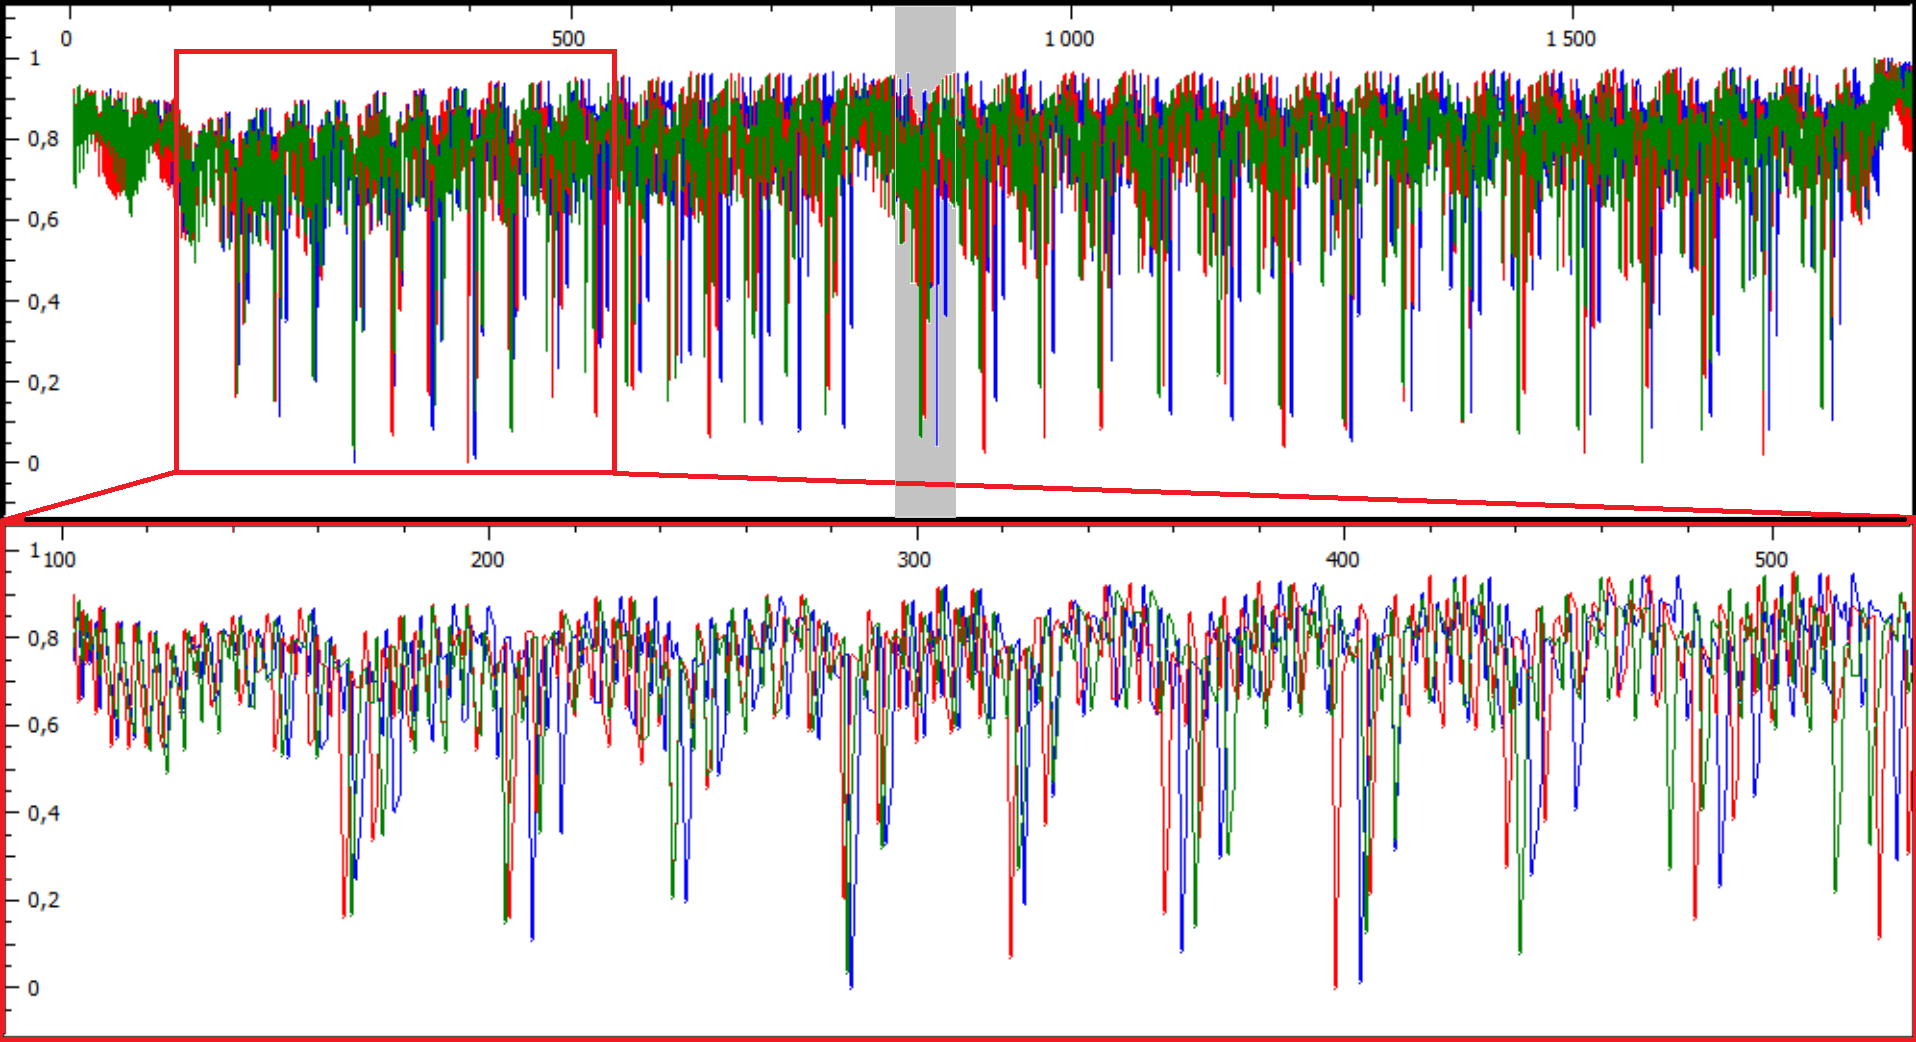
\includegraphics[width=\textwidth]{../Figures/CHES2017/jitter_2_2_framed.png} }
%\subfigure[]{\label{fig:jitter_traces66}
%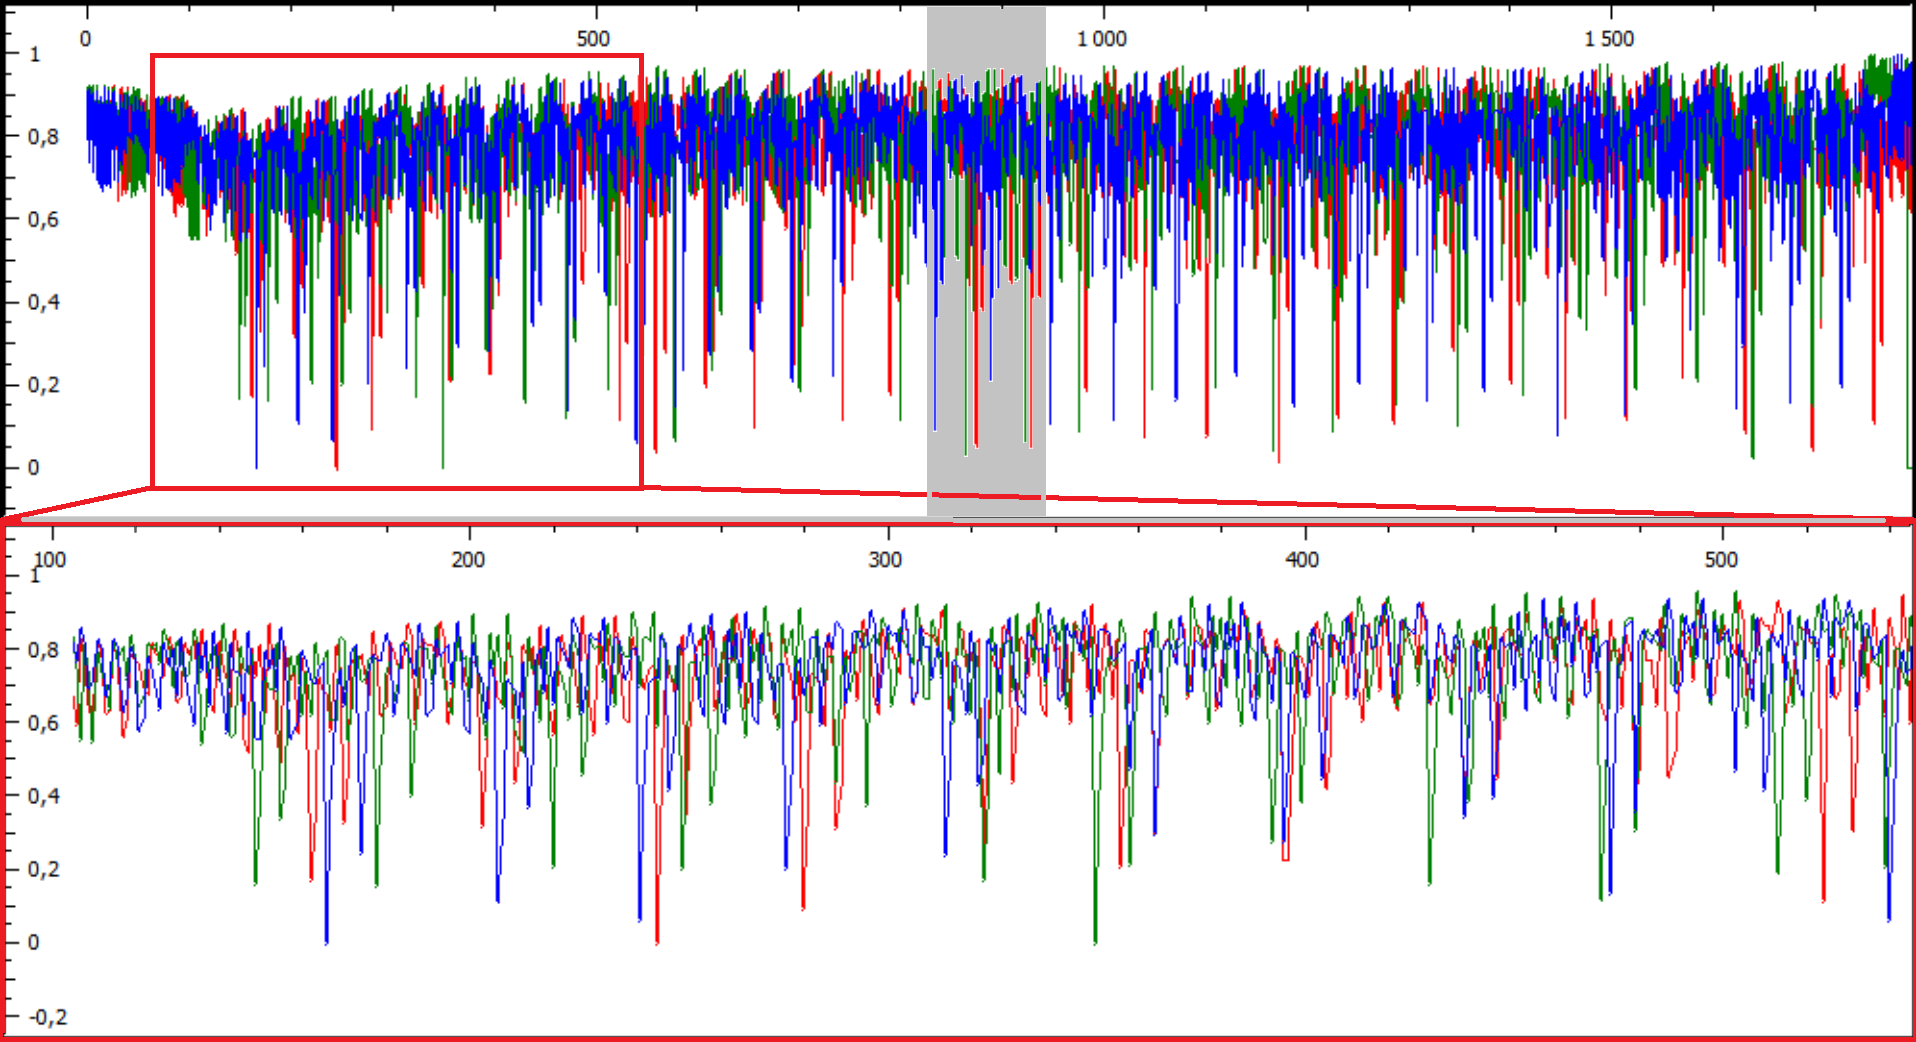
\includegraphics[width=\textwidth]{../Figures/CHES2017/jitter_6_6_framed.png} }
%\caption[Hardware misalignment: \emph{DS\_low\_jitter} and \emph{DS\_high\_jitter} datasets.]{\subref{fig:jitter_traces22}  some traces of the \emph{DS\_low\_jitter} dataset, a zoom of the part highlighted by the red rectangle is given in the bottom part. \subref{fig:jitter_traces22} some traces of the \emph{DS\_high\_jitter} dataset. The interesting clock cycle is highlighted by the grey rectangular area.}\label{fig:jitter_traces}
%\end{figure}


%
%\begin{figure}
%\centering
%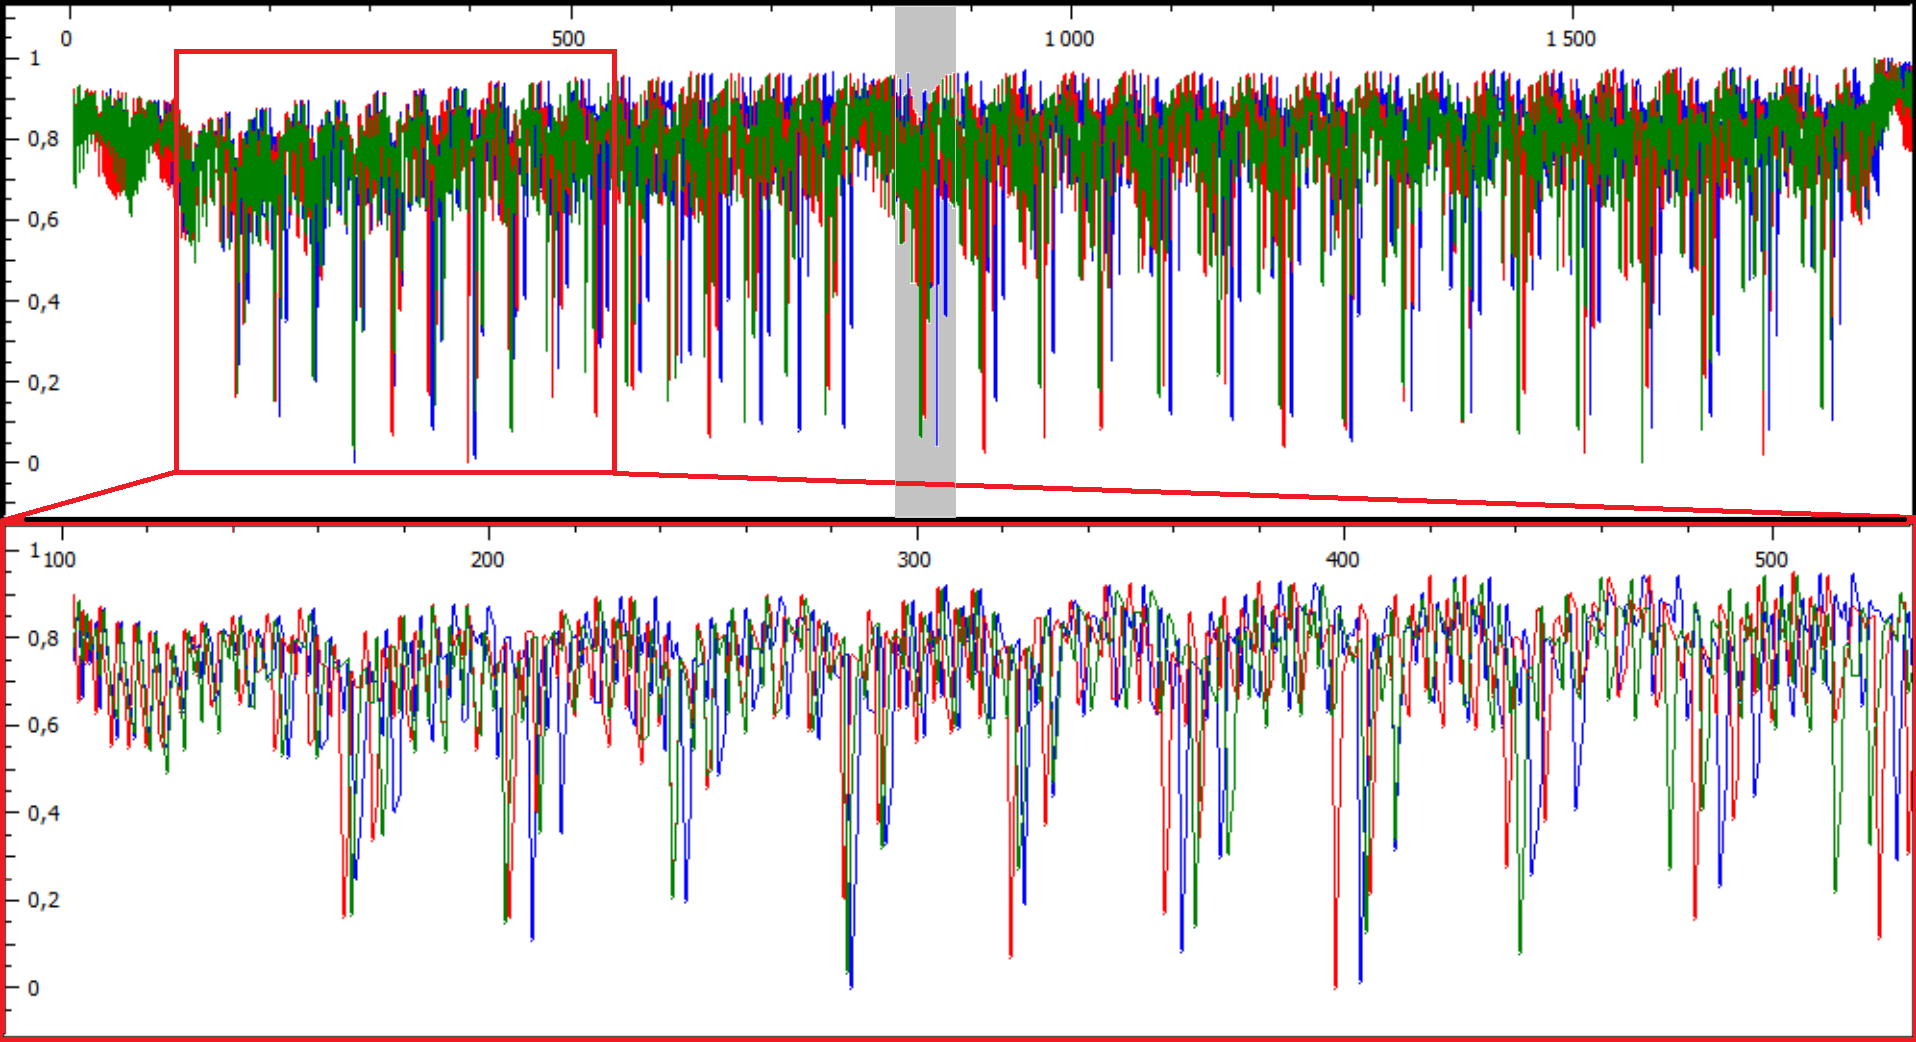
\includegraphics[width=.7\textwidth]{../Figures/CHES2017/jitter_2_2_framed.png} 
%\caption{Some traces of the \emph{DS\_low\_jitter} dataset, a zoom of the part highlighted by the red rectangle is given in the bottom part. }\label{fig:jitter_traces22}
%\end{figure}
%
%\begin{figure}
%\centering
%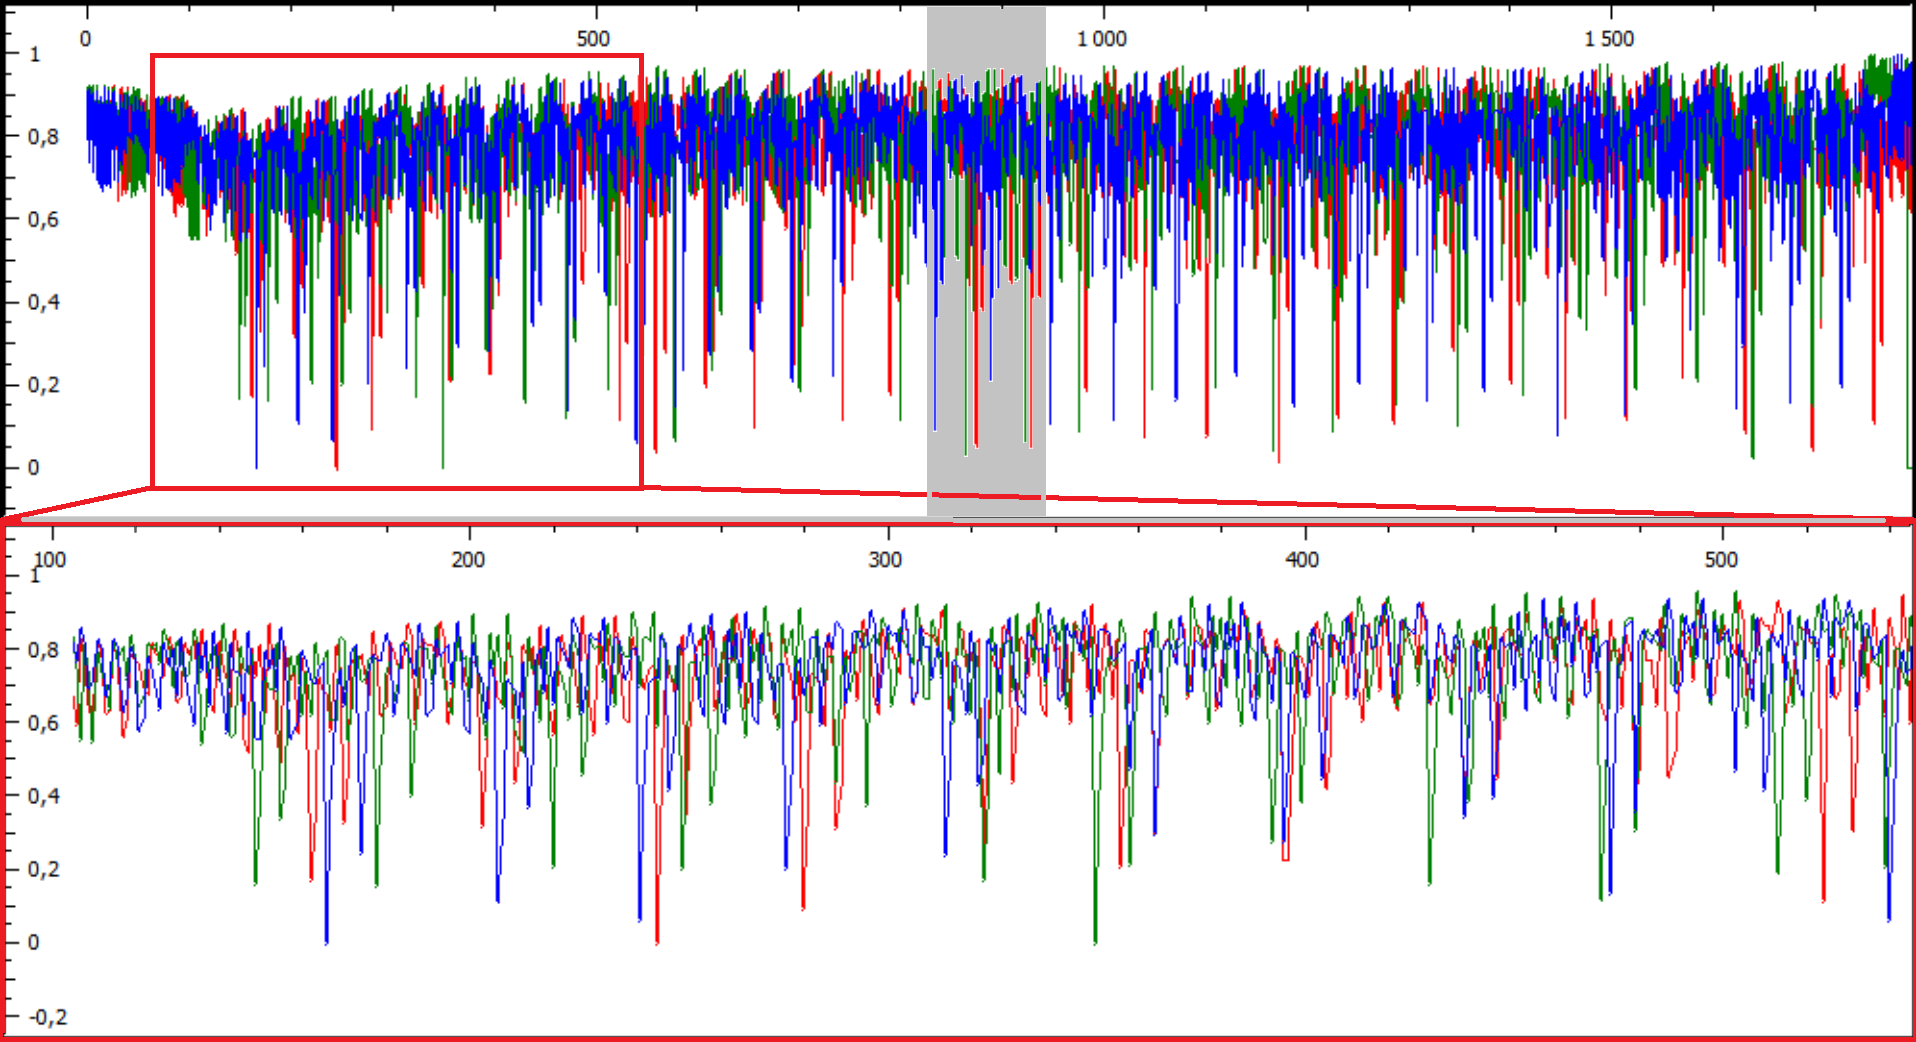
\includegraphics[width=.7\textwidth]{../Figures/CHES2017/jitter_6_6_framed.png} 
%\caption{Some traces (and the relative) of the \emph{DS\_high\_jitter} dataset. The interesting clock cycle is highlighted by the grey rectangular area.}\label{fig:jitter_traces66}
%\end{figure}


We used the same CNN architecture \eqref{eq:archi} as in previous section. We assisted again to a strong overfitting phenomenon and we successfully reduced it by applying the DA strategy introduced in Sec.~\ref{sec:DA}. This time we applied both the \emph{shifting} deformation $\mathrm{SH}_T$ with $T^\star = 200$ and $T\in\{0,20,40\}$ and the \emph{add-remove} deformation $\mathrm{AR}_R$ with $R\in \{0,100,200\}$, training the CNN model using the nine combinations $\mathrm{SH}_T\mathrm{AR}_R$. We performed a further experiment with much higher DA parameters, \ie $\mathrm{SH}_{200}\mathrm{AR}_{500}$, to show that the benefits provided by the DA are limited: as expected, too much deformation affects the CNN performances (indeed results obtained with $\mathrm{SH}_{200}\mathrm{AR}_{500}$ will be worse than those obtained with \eg $\mathrm{SH}_{40}\mathrm{AR}_{200}$).





The results we obtained are summarized in Table~\ref{table:results_all}. Case $\mathrm{SH}_0\mathrm{AR}_0$ corresponds to a training performed without DA technique, hence serves as a reference suffering from the overfitting phenomenon. It can be observed that as the DA parameters raise, the validation accuracy increases while the training accuracy decreases. This experimentally validates that the DA technique is efficient in reducing overfitting. Remarkably in some cases, for example in the \emph{DS\_low\_jitter} dataset case with $\mathrm{SH}_{100}\mathrm{AR}_{40}$, the best validation accuracy is higher than the best training accuracy. In Fig.~\ref{fig:high_acc} the training and validation accuracies achieved in this case epoch by epoch are depicted. It can be noticed that the unusual relation between the training and the validation accuracies does not only concern the maximal values, but is almost kept epoch by epoch. Observing the picture, we can be convinced that, since this fact occurs at many epochs, this is not a consequence of some unlucky inaccurate estimations. To interpret this phenomenon we observe that the training set contains both the original data and the augmented ones (\ie deformed by the DA) while the validation set only contains non-augmented data.  The fact that the achieved training accuracy  is lower than the validation one, indicates that the CNN does not succeed in learning how to classify the augmented data, but succeeds to extract the features of interest for the classification of the original data.  We judge this behaviour positively. Concerning the DA techniques we observe that they are efficient when applied independently and that their combination is still more efficient.

\begin{figure}[h]
\centering
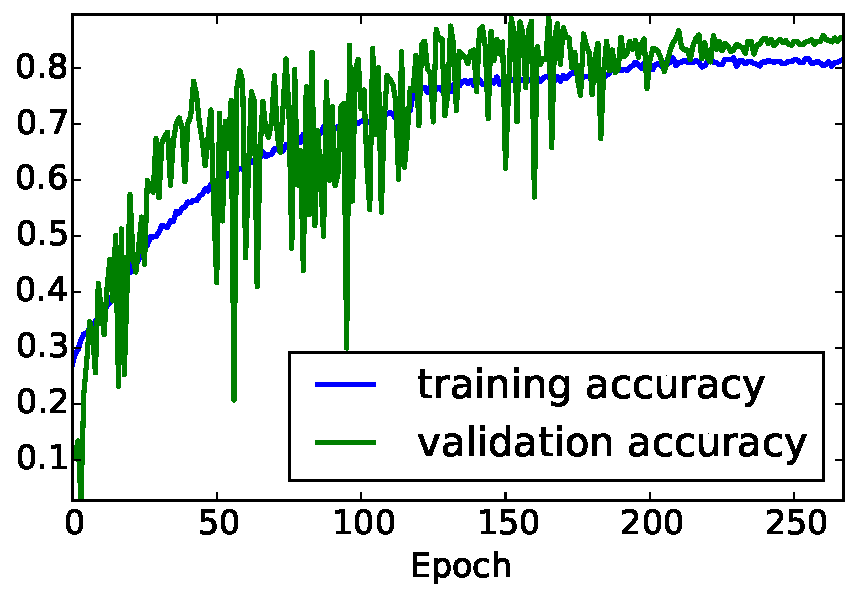
\includegraphics[width=.5\textwidth]{../Figures/CHES2017/acc_DAadd_remove100_shift_40_deep_good_for_CW_shift_wo_DO.pdf} 
\caption[Excessive Data Augmentation example.]{Training of the CNN model with DA $\mathrm{SH}_{100}\mathrm{AR}_{40}$. The training classification problem becomes harder than the real classification problem, leading validation accuracy constantly higher than the training one.}\label{fig:high_acc}
\end{figure}

\begin{figure}
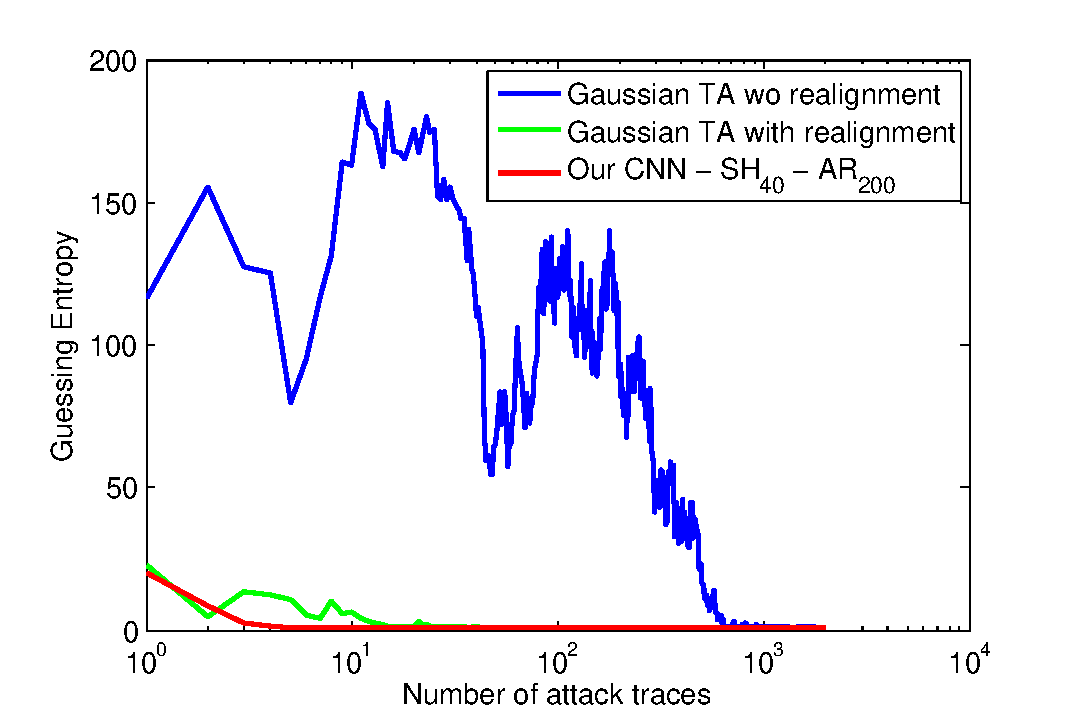
\includegraphics[width=.5\textwidth]{../Figures/CHES2017/results_low_jitter_new.pdf} 
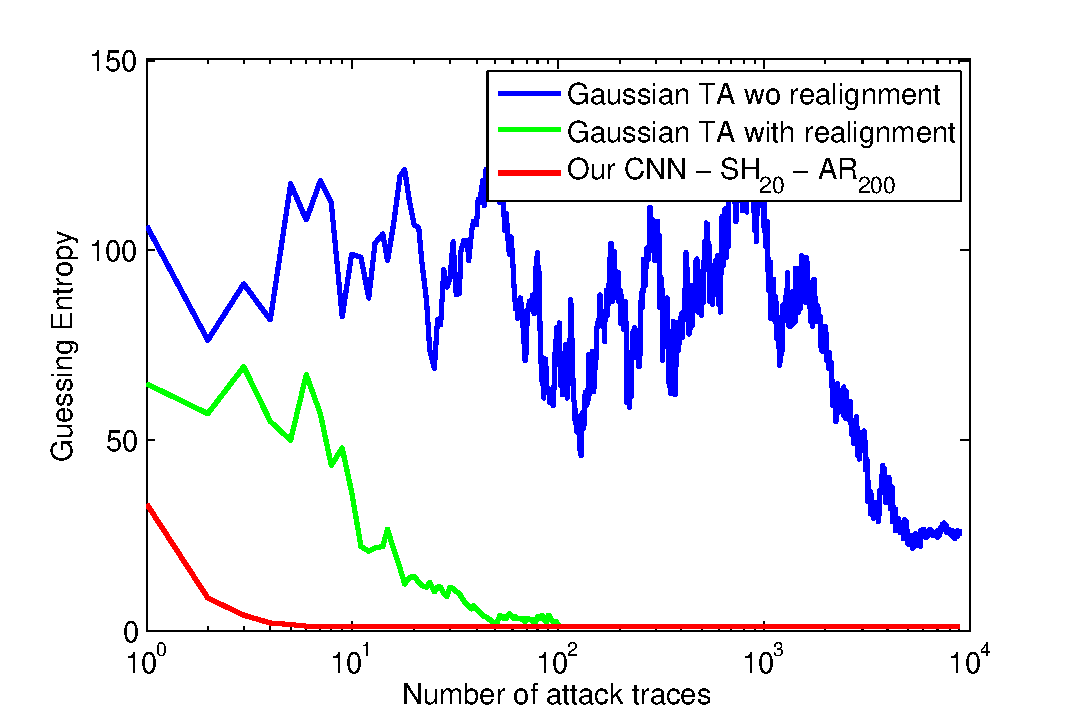
\includegraphics[width=.5\textwidth]{../Figures/CHES2017/results_high_jitter_new.pdf} 
\caption[Comparison between a Gaussian template attack, with and without realignment, and our CNN strategy, over the  \emph{DS\_low\_jitter} and the  \emph{DS\_high\_jitter}.]{Comparison between a Gaussian template attack, with and without realignment, and our CNN strategy, over the  \emph{DS\_low\_jitter} (left) and the  \emph{DS\_high\_jitter} (right).}\label{fig:compareTA}
\end{figure}



\newcolumntype{C}{>{\centering\arraybackslash}p{3em}}
\begin{table}[t]
\centering
\caption[Results of our CNN in presence of artificially-generated jitter countermeasure, with different DA techniques.]{Results of our CNN in presence of artificially-generated jitter countermeasure, with different DA techniques. See the caption of Table \ref{tab:res_CW_shift} for a legend.}
\label{table:results_all}



\begin{tabular}{|C|C|CCCCCC|CC}
\hline
\multicolumn{10}{|C|}{\textbf{\emph{DS\_low\_jitter}}}\\
\hline
$a$                           & $b$                         & \multicolumn{2}{C|}{}                                                                                      & \multicolumn{2}{C|}{}                                                                                     & \multicolumn{2}{C|}{}                                                                                  & \multicolumn{2}{C|}{}                                      \\ \cline{1-2}
$c$                           & $d$                         & \multicolumn{2}{C|}{\multirow{-2}{*}{$\mathrm{SH}_{0}$}}                                                   & \multicolumn{2}{c|}{\multirow{-2}{*}{$\mathrm{SH}_{20}$}}                                                 & \multicolumn{2}{c|}{\multirow{-2}{*}{$\mathrm{SH}_{40}$}}                                              & \multicolumn{2}{c|}{\multirow{-2}{*}{$\mathrm{SH}_{200}$}} \\ \hline
\multicolumn{2}{|c|}{}                                      & \multicolumn{1}{c|}{\cellcolor[HTML]{EFEFEF}100.0\%} & \multicolumn{1}{c|}{\cellcolor[HTML]{EFEFEF}68.7\%} & \multicolumn{1}{c|}{99.8\%}                         & \multicolumn{1}{c|}{86.1\%}                         & \multicolumn{1}{c|}{98.9\%}                                  & 84.1\%                                  &                              &                             \\ \cline{3-8}
\multicolumn{2}{|c|}{\multirow{-2}{*}{$\mathrm{AR}_{0}$}}   & \multicolumn{1}{c|}{\cellcolor[HTML]{EFEFEF}57.4\%}  & \multicolumn{1}{c|}{\cellcolor[HTML]{EFEFEF}14}     & \multicolumn{1}{c|}{82.5\%}                         & \multicolumn{1}{c|}{6}                              & \multicolumn{1}{c|}{83.6\%}                                  & 6                                       &                              &                             \\ \cline{1-8}
\multicolumn{2}{|c|}{}                                      & \multicolumn{1}{c|}{87.7\%}                          & \multicolumn{1}{c|}{88.2\%}                         & \multicolumn{1}{c|}{82.4\%}                         & \multicolumn{1}{c|}{88.4\%}                         & \multicolumn{1}{c|}{81.9\%}                                  & 89.6\%                                  &                              &                             \\ \cline{3-8}
\multicolumn{2}{|c|}{\multirow{-2}{*}{$\mathrm{AR}_{100}$}} & \multicolumn{1}{c|}{86.0\%}                          & \multicolumn{1}{c|}{6}                              & \multicolumn{1}{c|}{87.0\%}                         & \multicolumn{1}{c|}{5}                              & \multicolumn{1}{c|}{87.5\%}                                  & 6                                       &                              &                             \\ \cline{1-8}
\multicolumn{2}{|c|}{}                                      & \multicolumn{1}{c|}{83.2\%}                          & \multicolumn{1}{c|}{88.6\%}                         & \multicolumn{1}{c|}{81.4\%} & \multicolumn{1}{c|}{86.9\%} & \multicolumn{1}{c|}{\textbf{80.6\%}} &\textbf{88.9\%} &                              &                             \\ \cline{3-8}
\multicolumn{2}{|c|}{\multirow{-2}{*}{$\mathrm{AR}_{200}$}} & \multicolumn{1}{c|}{86.6\%}                          & \multicolumn{1}{c|}{6}                              & \multicolumn{1}{c|}{85.7\%} & \multicolumn{1}{c|}{6}      & \multicolumn{1}{c|}{\textbf{87.7\%}} & \textbf{5}      &                              &                             \\ \hline
\multicolumn{2}{|c|}{}                                      &                                                      &                                                     &                                                     &                                                     &                                                              &                                         & \multicolumn{1}{c|}{85.0\%}  & \multicolumn{1}{c|}{88.6\%} \\ \cline{9-10} 
\multicolumn{2}{|c|}{\multirow{-2}{*}{$\mathrm{AR}_{500}$}} &                                                      &                                                     &                                                     &                                                     &                                                              &                                         & \multicolumn{1}{c|}{86.2\%}  & \multicolumn{1}{c|}{5}      \\ \cline{1-2} \cline{9-10}
\multicolumn{10}{|C|}{}\\
\hline
\multicolumn{10}{|C|}{\textbf{\emph{DS\_high\_jitter}}}\\
\hline
$a$                          & $b$                         & \multicolumn{2}{C|}{\multirow{2}{*}{$\mathrm{SH}_{0}$}}   & \multicolumn{2}{C|}{\multirow{2}{*}{$\mathrm{SH}_{20}$}}  & \multicolumn{2}{C|}{\multirow{2}{*}{$\mathrm{SH}_{40}$}} & \multicolumn{2}{C|}{\multirow{2}{*}{$\mathrm{SH}_{200}$}} \\ \cline{1-2}
$c$                          & $d$                         & \multicolumn{2}{C|}{}                                     & \multicolumn{2}{C|}{}                                     & \multicolumn{2}{C|}{}                                    & \multicolumn{2}{C|}{}                                     \\ \hline
\multicolumn{2}{|C|}{\multirow{2}{*}{$\mathrm{AR}_{0}$}}   & \multicolumn{1}{C|}{\cellcolor[HTML]{EFEFEF}100\%}  & \multicolumn{1}{l|}{\cellcolor[HTML]{EFEFEF}45.0\%} & \multicolumn{1}{C|}{100\%}  & \multicolumn{1}{C|}{60.0\%} & \multicolumn{1}{l|}{98.5\%}           & 67.6\%           &                             &                             \\ \cline{3-8}
\multicolumn{2}{|C|}{}                                     &  \multicolumn{1}{C|}{\cellcolor[HTML]{EFEFEF}40.6\%} & \multicolumn{1}{C|}{\cellcolor[HTML]{EFEFEF}35}  & \multicolumn{1}{C|}{51.1\%} & \multicolumn{1}{C|}{9}      & \multicolumn{1}{C|}{62.4\%}           & 11               &                             &                             \\ \cline{1-8}
\multicolumn{2}{|C|}{\multirow{2}{*}{$\mathrm{AR}_{100}$}} & \multicolumn{1}{C|}{90.4\%} & \multicolumn{1}{l|}{57.3\%} & \multicolumn{1}{C|}{76.6\%} & \multicolumn{1}{C|}{73.6\%} & \multicolumn{1}{C|}{78.5\%}           & 76.4\%           &                             &                             \\ \cline{3-8}
\multicolumn{2}{|C|}{}                                     & \multicolumn{1}{C|}{50.2\%} & \multicolumn{1}{C|}{15}     & \multicolumn{1}{C|}{72.4\%} & \multicolumn{1}{C|}{11}     & \multicolumn{1}{C|}{73.5\%}           & 9                &                             &                             \\ \cline{1-8}
\multicolumn{2}{|C|}{\multirow{2}{*}{$\mathrm{AR}_{200}$}} & \multicolumn{1}{C|}{83.1\%} & \multicolumn{1}{C|}{67.7\%} &\multicolumn{1}{C|}{\textbf{82.0\%}} & \multicolumn{1}{C|}{\textbf{77.1\%}} & \multicolumn{1}{l|}{82.6\%}           & 77.0\%           &                             &                             \\ \cline{3-8}
\multicolumn{2}{|C|}{}                                     & \multicolumn{1}{C|}{64.0\%} & \multicolumn{1}{C|}{11}     & \multicolumn{1}{C|}{\textbf{75.5\%}} & \multicolumn{1}{C|}{\textbf{8}}   & \multicolumn{1}{C|}{74.4\%}           & 8                &                             &                             \\ \hline
\multicolumn{2}{|C|}{\multirow{2}{*}{$\mathrm{AR}_{500}$}} &                             &                             &                             &                             &                                       &                  & \multicolumn{1}{C|}{83.6\%} & \multicolumn{1}{C|}{73.4\%} \\ \cline{9-10} 
\multicolumn{2}{|C|}{}                                     &                             &                             &                             &                             &                                       &                  & \multicolumn{1}{C|}{68.2\%} & \multicolumn{1}{C|}{11}     \\ \cline{1-2} \cline{9-10}  
\end{tabular}


\end{table}
According to our results in Table~\ref{table:results_all}, we selected the model issued using the $\mathrm{SH}_{200}\mathrm{AR}_{40}$ technique for the \emph{DS\_low\_jitter} dataset and the one issued using the $\mathrm{SH}_{200}\mathrm{AR}_{20}$ technique for the \emph{DS\_higher\_jitter}. In Fig.~\ref{fig:compareTA} we compare their performances with those of a Gaussian TA combined with a realignment technique. To tune this comparison, several state-of-the-art  Gaussian TA have been tested. Since in the experiment the leakage is concentrated in peaks that are easily detected by their relatively high amplitude, we use as realignment technique a simple method that consists in first detecting the peaks above a chosen threshold, then keeping all the samples in a window around these peaks. Then, for the selection of the PoIs, two approaches have been applied: first we selected from $3$ to $20$ points maximising the estimated instantaneous SNR, secondly we selected sliding windows of 3 to 20 consecutive points covering the region of interest. For the template processing, we tried (1) the classical approach \cite{Chari2003} where a mean and a covariance matrix are estimated for each class, (2) the \emph{pooled} covariance matrix strategy proposed in \cite{choudary2014efficient} and (3) the stochastic approach proposed in \cite{schindler2005stochastic}. The results plotted in Fig.~\ref{fig:compareTA} are the best ones we obtained (via the stochastic approach over some 5-sized windows). Results show that the performances of the CNN approach are much higher than those of the Gaussian templates, both with and without realignment. This confirms the robustness of the CNN approach with respect to the jitter effect:
the selection of PoIs and the realignment integrated in the training phase are effective.



\section{Experiments against Real-Case Hardware Countermeasures}\label{sec:AES}
As a last (but most challenging) experiment we deployed our CNN architecture to attack an AES hardware implementation over a modern secure smartcard (secure implementation on 90nm technology node). On this implementation, the architecture is designed to optimise the area, and the speed performances are not the major concern. The architecture is here minimal, implementing only one hardware instance of the SubByte module.  The AES SubByte operation is thus executed serially and one byte is processed per clock cycle. To protect the implementation, several countermeasures are implemented.  Among them, a hardware mechanism induces a strong jitter effect which produces an important traces' desynchronisation. The bench is set up to trig the acquisition of the trace on a peak which corresponds to the processing of the first byte. Consequently, the set of traces is aligned according to the processing of the first byte while the other bytes leakages are completely misaligned. To illustrate the effect of this misalignment, the SNR characterising the (aligned) first byte and the (misaligned) second byte are computed (according to \eqref{eq:SNR_formula}) using a set of $150,000$ traces labelled by the value of the SubByte output (256 labels). These SNRs are depicted in the top part of Fig.~\ref{fig:SNR}. The SNR of the first byte (in green) detects a quite high leakage, while the SNR of the second byte (in blue) is nullified. A zoom of the SNR of the second peak is proposed in the bottom part of Fig.~\ref{fig:SNR}. In order to confirm that the very low SNR corresponding to the second byte is only due to the desynchronisation, the patterns of the traces corresponding to the second byte have been resynchronised using a peak-detection-based algorithm, quite similar to the one applied for the experiments of Sec.~\ref{sec:artificial}. Then the SNR has been computed onto these new aligned traces and has been plot in red in the top-left part of Fig.~\ref{fig:SNR}; this SNR is very similar to that of the first byte. This clearly shows that (1) the leakage information is contained into the trace but is efficiently hidden by the jitter-based countermeasure, and that (2) the realignment technique we applied in this context is effective.

We applied the CNN approach onto the rough set of traces (without any alignement). First, a $2,500$-long window of the trace has been selected to input CNN. The window, identified by the vertical cursors in the bottom part of Fig.~\ref{fig:SNR}, has been selected to ensure that the pattern corresponding to the leakage of the second byte is inside the selection. At this step, it is important to notice that such a selection is not at all  as meticulous as the selection of PoIs required by a classical TA approach. The training phase has been performed using $98,000$ labelled traces; $1,000$ further traces have been used for the validation set. We performed the training phase over a desktop computer equipped with an Intel Xeon E5440 @2,83GHz processor, 24Gb of RAM and a GeForce GTS 450 GPU. Without data augmentation each epoch took about 200s.\footnote{raising to about $2,000$ seconds when $SH_{20}DA_{200}$ data augmentation is performed (data are augmented online during training)} The training stopped after 25 epochs. Considering that in this case we applied an early-stopping strategy that stopped training after 20 epochs without validation loss decrement, it means that the final trainable weights are obtained after 5 epochs (in about 15 minutes). The results that we obtained are summarized in Table~\ref{tab:res_AES}. They prove not only that our CNN is robust to the misalignment caused by the jitter but also that the DA technique is effective in raising its efficiency. A comparison between the CNN performances and the best results we obtained over the same dataset applying the realignment-TA strategy, is proposed in Fig.~\ref{fig:TA_smartcard}. Beyond the fact that the CNN approach slightly outperforms the realignment-TA one, and considering that both case-results shown here are surely non-optimal, what is remarkable is that the CNN approach is potentially suitable even in cases where realignment methods are impracticable or not satisfying. It is of particular interest in cases where sensitive information does not lie in proximity of peaks or of easily detectable patterns, since many resynchronisation techniques are based on pattern or peak detection. If the resynchronisation fails, the TA approach falls out of service, while the CNN one remains a further weapon in the hands of an attacker.

\begin{figure}
    \centering
    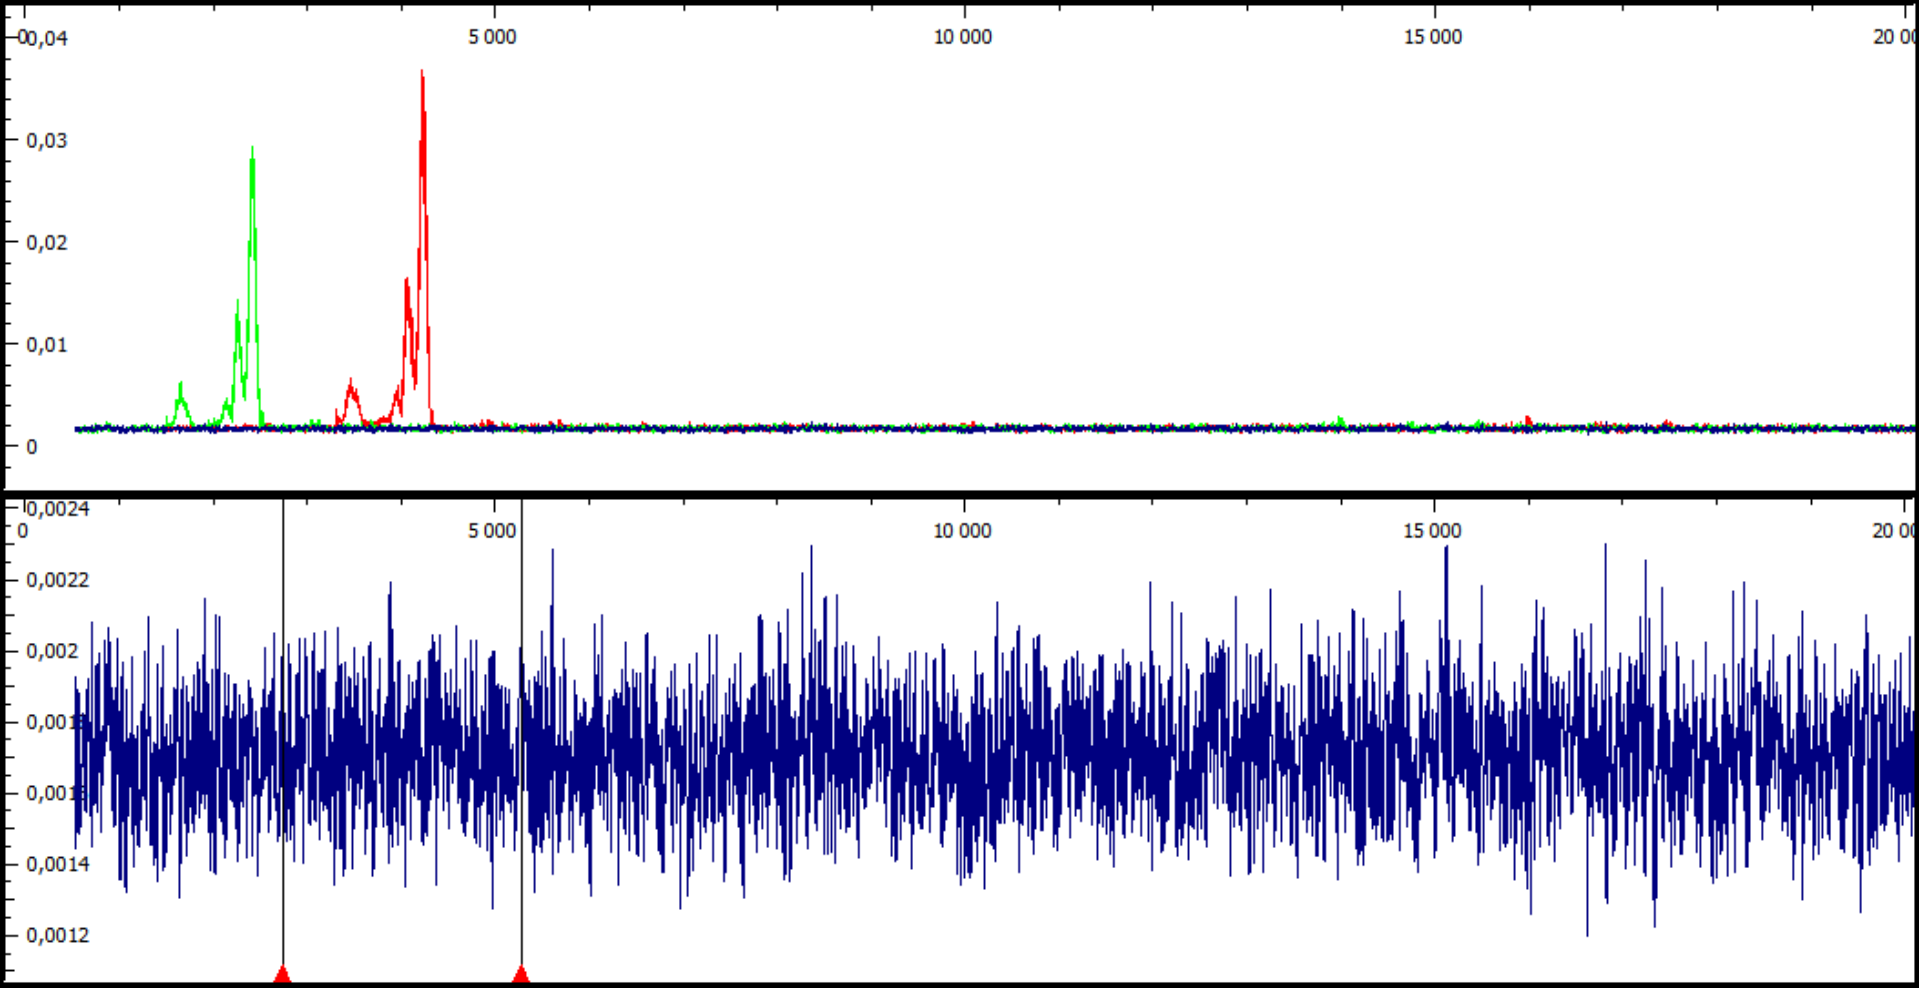
\includegraphics[width=\textwidth]{../Figures/CHES2017/snrs.png} 
     \caption[SNR values for an AES hardware implementation protected by jitter-based misalignment.]{AES hardware implementation protected by jitter-based misalignment. In green the SNR for the first byte; in blue the SNR for the second byte; in red the SNR for the second byte after a trace realignment.}\label{fig:SNR}
\end{figure}


\begin{figure}
    \centering
    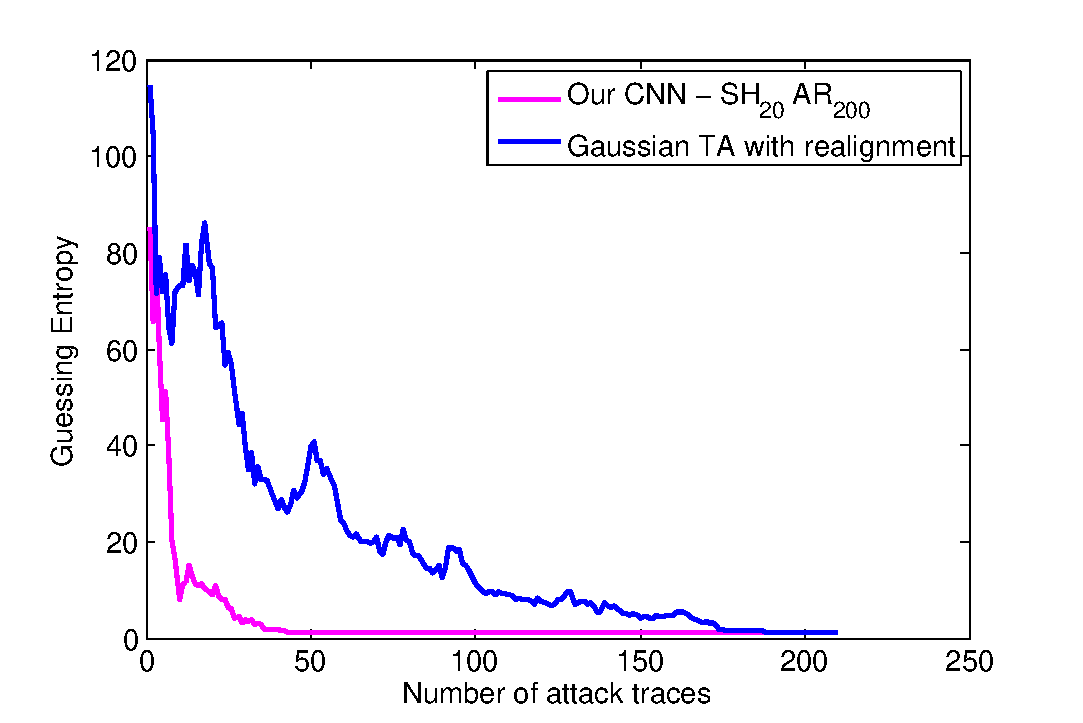
\includegraphics[width=\textwidth]{../Figures/CHES2017/TA_CNN_smartcard.pdf} 
     \caption{Comparison between a Gaussian template attack with realignment, and our CNN strategy, over the modern smart card with jitter.}\label{fig:TA_smartcard}
\end{figure}

%
%    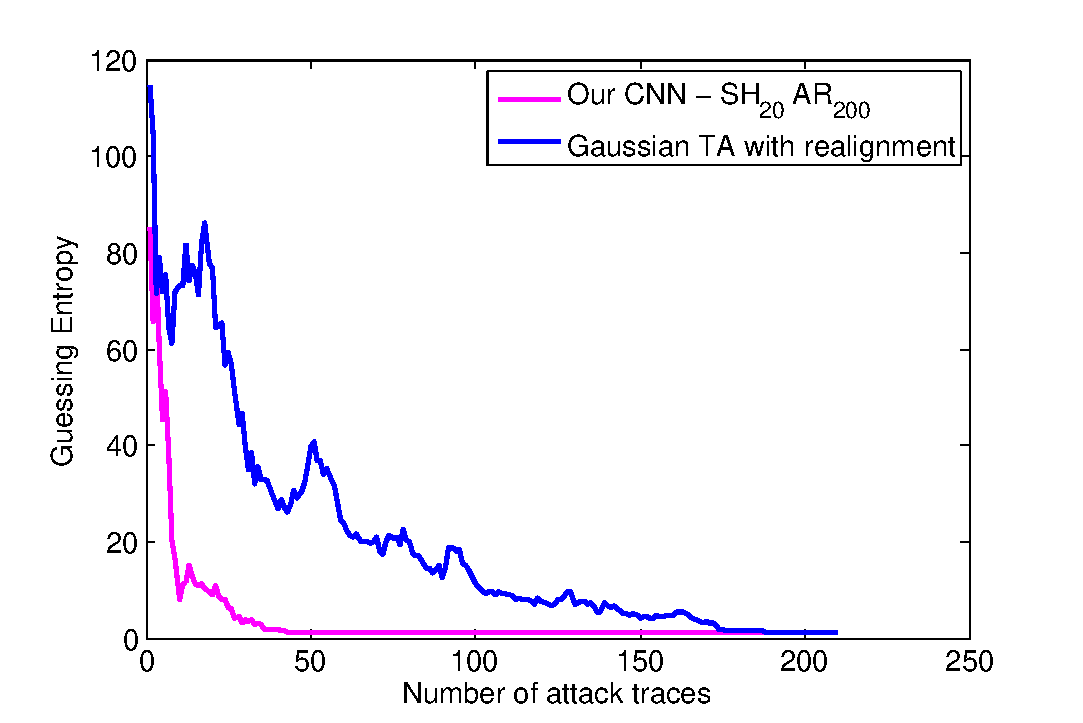
\includegraphics[width=.45\textwidth]{../Figures/CHES2017/TA_CNN_smartcard.pdf} 
%    \captionof{figure}{Top Left: in green the SNR for the first byte; in blue the SNR for the second byte; in red the SNR for the second byte after a trace realignment. Bottom Left: a zoom of the blue SNR trace. Right: comparison between a Gaussian template attack with realignment, and our CNN strategy, over the modern smart card with jitter.}\label{fig:SNR}

    

\begin{table}
\centering
\begin{tabular}{|c|c|c|c|c|c|c|c|}
\multicolumn{8}{c}{}\\
\hline
\multicolumn{2}{|c|}{} & \multicolumn{2}{c|}{$\mathrm{SH}_{0}\mathrm{AR}_{0}$} & \multicolumn{2}{c|}{$\mathrm{SH}_{10}\mathrm{AR}_{100}$} & \multicolumn{2}{c|}{$\mathrm{SH}_{20}\mathrm{AR}_{200}$} \\ \hline
$a$        & $b$       & 35.0\%                     & 1.1\%                    & 12.5\%                      & 1.5\%                      & \textbf{10.4\%}             & \textbf{2.2\%}             \\ \hline
$c$        & $d$       & 1.2\%                      & 137                      & 1.3\%                       & 89                         & \textbf{1.8\%}              & \textbf{54}                \\ \hline
\end{tabular}

\caption{Results of our CNN over the modern smart card with jitter.}\label{tab:res_AES}
\end{table}

  
\section{Conclusion}
In this chapter, we have proposed an end-to-end profiling attack approach, based on the CNNs. We claimed that such a strategy would keep effective even in presence of trace misalignment, and we successfully verified our claim by performing CNN-based attacks against different kinds of misaligned data. This property represents a great practical advantage compared to the state-of-the-art Template Attacks, that require a meticulous trace realignment in order to be efficient. Our strategy based over CNNs differs from classical TA for mainly two points. First, it makes use of a discriminative model, instead of a generative one. Second it takes in charge into a unique training phase all eventual preprocessing phases necessary for the successfulness of a TA. Indeed, beyond the trace realignment, that is not necessary for the CNN approach, it represents as well a solution to the problem of the selection of points of interest issue: CNNs efficiently manage high-dimensional data, allowing the attacker to simply  select large windows. In this sense, the experiments described in Sec.~\ref{sec:AES} are very representative: our CNN retrieves information from a large window of points instead of an almost null instantaneous SNR. To guarantee the robustness to trace misalignment, we used a quite complex architecture for our CNN, and we clearly identified the risk of overfitting phenomenon. To deal with this classical issue in machine learning, we proposed two Data Augmentation techniques adapted to misaligned side-channel traces. All the experimental results we obtained have proved that they provide a great benefit to the CNN strategy.  Attacks proposed in this chapter are performed against non-masked implementation. Nevertheless, since NNs are in general non-linear models, they naturally well-fit also the higher-order attack context, as discussed in \cite{maghrebi2016breaking} and \cite{DLwhitepaper}.